\documentclass[aps,floatfix,10pt,amssymb,amsfont,amsmath,superscriptaddress,float,nofootinbib,longbibliography,nobalancelastpage,twocolumn]{revtex4-2}
\usepackage{graphicx} % Required for inserting images
\usepackage{hyperref}
\usepackage{braket}
\usepackage{amsfonts}
\usepackage{amssymb}
\usepackage{amsmath}
\usepackage{bbm}
\usepackage{bm}
\usepackage[english]{babel}
\usepackage{amsthm}
\newtheorem{theorem}{Theorem}
\newtheorem{lemma}{Lemma}
\newtheorem{duplicate}{Theorem}
\newtheorem{corollary}{Corollary}
\usepackage{subfig}
\usepackage{tikz}
\usetikzlibrary{arrows,positioning}
 \usetikzlibrary{quotes}
\usepackage{yquant}
\pgfdeclareshape{yquant-multictrlshape}{
   \inheritsavedanchors[from=yquant-circle]%
   \foreach \anc in {center, north, north east, east, south east, south, south west, west, north west} {%
      \inheritanchor[from=yquant-circle]{\anc}%
   }%
   \inheritanchorborder[from=yquant-circle]%
   \backgroundpath{%
      \pgfpathmoveto{\pgfqpoint{-0.707107\dimexpr\xradius\relax}{-0.707107\dimexpr\yradius\relax}}%
      \pgfpathlineto{\pgfqpoint{0.707107\dimexpr\xradius\relax}{0.707107\dimexpr\yradius\relax}}%
      \pgfpathellipse{\pgfpointorigin}%
                     {\pgfqpoint{\xradius}{0pt}}%
                     {\pgfqpoint{0pt}{\yradius}}%
   }%
   \inheritclippath[from=yquant-circle]%
}

\yquantset{multictrl/.style={every negative control/.style={draw, /yquant/default fill,shape=yquant-multictrlshape,radius=1.05mm}}}
\pgfdeclareshape{yquant-bctrlshape}{
   \inheritsavedanchors[from=yquant-circle]%
   \foreach \anc in {center, north, north east, east, south east, south, south west, west, north west} {%
      \inheritanchor[from=yquant-circle]{\anc}%
   }%
   \inheritanchorborder[from=yquant-circle]%
   \backgroundpath{%
      % Draw the circle
      \pgfpathellipse{\pgfpointorigin}%
                     {\pgfqpoint{\xradius}{0pt}}%
                     {\pgfqpoint{0pt}{\yradius}}%
   }%
   % Add the "b" in the center
   \foregroundpath{%
      \pgftext[center]{\(\scriptstyle b\)}%
   }%
   \inheritclippath[from=yquant-circle]%
}

\yquantset{
  bctrl/.style={
    every control/.style={
      draw,
      /yquant/default fill,
      shape=yquant-bctrlshape,
      radius=1.05mm
    }
  }
}
\date{February 2025}
\begin{document}
\yquantdefinebox{dots}[inner sep=0pt]{$\dots$}

\title{New and Improved Quantum Metropolis Sampling}
\author{Oliver O'Brien}
\affiliation{Department of Applied Mathematics and Theoretical Physics, University of Cambridge,\\ Wilberforce Road, Cambridge, CB3 0WA, United Kingdom}
\author{Rakesh Achutha}
\affiliation{Department of Applied Mathematics and Theoretical Physics, University of Cambridge,\\ Wilberforce Road, Cambridge, CB3 0WA, United Kingdom}
\author{Frank Verstraete}
\affiliation{Department of Applied Mathematics and Theoretical Physics, University of Cambridge,\\ Wilberforce Road, Cambridge, CB3 0WA, United Kingdom}
\affiliation{Department of Physics and Astronomy, Ghent University, Krijgslaan 281, 9000 Gent, Belgium}

\begin{abstract}
    We introduce a resource-efficient protocol for Boosted State-Independent Quantum Phase Estimation (BSI-QPE), enabling practical implementation of the Quantum Metropolis algorithm. By employing window functions to suppress fat tails, our approach maintains coherence and shift invariance required for reversible sampling. We reframe the rejection process using a two-dimensional invariant subspace. A modified formulation of approximate quantum detailed balance is proposed, ensuring convergence to Gibbs states under realistic error bounds. These advancements significantly lower the resource threshold for quantum thermal state preparation.
\end{abstract}

\maketitle

\section{Introduction}
The Quantum Metropolis algorithm, first proposed by Temme et al. \cite{Temme_2011}, remains one of the most promising quantum algorithms for sampling from Gibbs (thermal) states of quantum systems. These states are fundamental in statistical mechanics and appear across condensed matter physics, quantum chemistry, and high-energy physics, where accurate thermal state preparation is a central computational challenge. 

However, the algorithm as originally stated suffers from two major issues which have led the community to investigate alternative gibbs sampling techniques (\cite{}). Firstly, \cite{Temme_2011} heavily relies upon phase estimation and hence has to deal with the resultant fat tails \cite{}.  Numerous solutions to this problem have been explored (\cite{}). In the original paper \cite{Temme_2011} it was posited that coherently taking the median of multiple phase estimations could help boost the signal and remove these fat tails. However, the phase estimation is also required to be shift invariant which the median trick struggles to fulfill. Recently, \cite{chen2023quantumthermalstatepreparation} proved a no-go theorem suggesting that it is not possible to implement the boosted shift-invariant phase estimation required by the quantum metropolis algorithm. 

We propose a boosted shift-invariant phase estimation protocol which utilises window functions to exponentially dampen the fat tails. This drastically reduces the number of ancilla qubits required for the algorithm to work, and also conclusively proves that quantum metropolis does indeed work. 

In Section \ref{section:boostedphaseestimation} we present the construction of the Boosted Shift-Invariant Quantum Phase Estimation (BSI-QPE) protocol, including a detailed circuit-level description and error analysis based on window functions. In Section \ref{section:algorithm}, we describe our modified Quantum Metropolis algorithm incorporating our improved quantum phase estimation. This includes a novel understanding of the rewinding mechanism formulated through iterative projective measurements and invariant subspaces. Section \ref{section:why} rigorously proves that our algorithm satisfies an approximate quantum detailed balance condition and discusses the convergence guarantees to the thermal Gibbs state. Finally, in Section \ref{section:discussion}, we discuss the broader implications of our results, the assumptions made, and the outlook for implementing these techniques on near-term or fault-tolerant quantum hardware.


\section{Boosted State-Independent Quantum Phase Estimation}
\label{section:boostedphaseestimation}
Given an $m$-qubit Hamiltonian $H$ eigenvectors $\ket{\psi_j}$ such that $H\ket{\psi_j} = E_j \ket{\psi_j}$, quantum phase estimation (QPE) allows one to prepare an ancilla register that approximates $E_j$. Unfortunately, quantum computers have limited precision. As a result, unless the energy can be represented exactly in binary using $\eta$ bits (corresponding to $\eta$ ancilla qubits), there is a high probability of obtaining an inaccurate energy measurement. This inaccuracy arises from the ``fat tails" in QPE \cite{}. 

Often this issue can be mitigated by simply repeating the calculation and taking an average. However, quantum metropolis sampling requires us to ``rewind" upon rejecting a proposed update and hence we require a unitary method for ``boosting" QPE. This ``boosted" QPE stores an approximation to the energy in ancillas which is not immediately measured but rather used as the basis for further coherent calculations. Further, for ``rewinding" to work we must reuse the same ancilla registers so the QPE protocol must also be state-independent. Therefore, we must demonstrate an implementation of a boosted state-independent quantum phase estimation (BSI-QPE). While it has been shown \cite{chen2023quantumthermalstatepreparation} that QPE cannot entirely eliminate the probability mass in its tails, we demonstrate that it is possible to construct BSI-QPE protocols with exponentially suppressed tails, which effectively mitigate the issue for practical purposes. 

Existing methods for boosting QPE rely upon choosing specific input ancillary states. In these methods QPE is performed using ancillas initialised to the normalized state $\sum_x \alpha(x) \ket{x}$ for some window function $\alpha(x)$ instead of the standard uniform superposition. In the following introductory Fourier formula, $E_j$ denotes the corresponding dimensionless phase. After performing QPE upon eigenstate $\ket{\psi_j}$ the following state is produced:
\begin{equation}
   \frac{1}{\sqrt{2^{\eta}}} \sum_x \sum_k e^{\frac{2 \pi i}{2^{\eta}}x(k-E_j)} \alpha(x)\ket{k}\ket{\psi_j}
\end{equation}
which can be rewritten as:
\begin{equation}
    \sum_k \hat\alpha(k-E_j) \ket{k}\ket{\psi_j}
\end{equation}
where $\hat \alpha(k)$ is the discrete fourier transform of $\alpha(x)$. By choosing $\alpha$ to be a window function one can ensure that $\hat \alpha$ is narrowly peaked, thus QPE is boosted. Unfortunately, this is not sufficient for the quantum metropolis algorithm as we require the QPE to be independent of the ancillary state, as we must reuse the same ancillas throughout the rewinding process. 

Our construction uses two window functions $\alpha(x)$ and $\beta(x) = \sqrt{1-\alpha(x)^2}$ (for $x\in\{0,1,\ldots,2^{\eta}-1\}$) which are both narrowly peaked in the fourier domain. We introduce these windows via the following multi-controlled single-qubit rotation:
\begin{equation}
   CR_Y = \sum_k \ket{k}\bra{k}\otimes \begin{pmatrix}
        \alpha(k)& \beta(k)\\
        -\beta(k)& \alpha(k)
    \end{pmatrix}
\end{equation}

We also require the following time evolution gadget which is constructed as shown in Fig~\ref{fig:CRZ}:
\begin{equation}
    CR_Z =\sum_{j,k}\ket{\psi_j}\bra{\psi_j}\otimes\ket{k}\bra{k} \otimes \begin{pmatrix}
        e^{\frac{iE_jkt}{2}}&0\\
        0 & e^{-\frac{iE_jkt}{2}}
    \end{pmatrix}
\end{equation}
\begin{figure*}
\[
\vcenter{\hbox{
\resizebox{!}{2.5cm}{
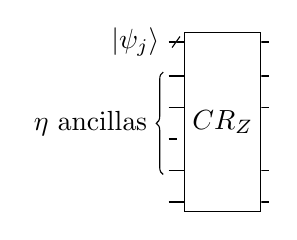
\begin{tikzpicture}
\begin{yquant*}
qubit {$\ket{\psi_j}$} s;

init {$\eta$ ancillas} (a[0,1],ellipsis, aend);
slash s;
hspace {0.1cm} -;
discard ellipsis;
% qubit {} aend;
qubit {} f;
box {$CR_Z$} (s,a,ellipsis, aend, f);

% text {$\ket{0}$} f;
\end{yquant*}
\end{tikzpicture}}}}
=
\vcenter{\hbox{
\resizebox{!}{2.5cm}{
    \begin{tikzpicture}
\begin{yquant*}
qubit {$\ket{\psi_j}$} s;

init {$\eta$ ancillas} (a[0,1],ellipsis, aend);
discard ellipsis;
% qubit {} aend;
qubit {} f;
slash s;
hspace {0.1cm} -;

box {$U^{\dagger 2^0}$} (s) | a[0], f;
box {$U^{\dagger 2^1}$} (s) | a[1], f;
hspace {0mm} -;
dots ellipsis;

box {$U^{\dagger 2^{\eta-1}}$} (s) | aend[0], f;
box {$U^{2^0}$} (s) | a[0]~ f;
box {$U^{ 2^1}$} (s) | a[1]~ f;
hspace {0mm} -;
dots ellipsis;

box {$U^{ 2^{\eta-1}}$} (s) | aend[0]~ f;
\end{yquant*}
\end{tikzpicture}}}}
\]
\caption{Quantum circuit for implementing an $Z$ rotation on an ancilla qubit that is dependent upon the energy of the system. The unitary $U=e^{\frac{iHt}{2}}$ is implemented through some quantum time evolution algorithm (e.g. trotterisation \cite{lloyd1996universal}, qubitization \cite{Low2019hamiltonian}) up to an operator norm error of $\epsilon^T_t$. Throughout this work we assume  $\epsilon^T_t$ is negligible, and use perfect quantum time evolution in our error analysis.}
    \label{fig:CRZ}
\end{figure*}
Both of these act as controlled $R_Z$ and $R_Y$ rotations on a single qubit. 
\begin{figure*}
\[
\vcenter{\hbox{
\resizebox{!}{2.5cm}{
\begin{tikzpicture}
    \begin{yquant*}
qubit {$\ket{\psi_j}$} s;

init {$\eta$ ancillas} (a[0,1],ellipsis, aend);
slash s;
% hspace {0.1cm} -;
discard ellipsis;
% qubit {} aend;
qubit {} f;
dots ellipsis;

box {BSI-\\QPE} (s,a,ellipsis, aend, f);

% text {$\ket{0}$} f;
\end{yquant*}
\end{tikzpicture} }}}
=
\vcenter{\hbox{
\resizebox{!}{2.5cm}{
\begin{tikzpicture}
    \begin{yquant*}
qubit {$\ket{\psi_j}$} s;

init {$\eta$ ancillas} (a[0,1],ellipsis, aend);
slash s;
discard ellipsis;
% qubit {} aend;
qubit {} f;
dots ellipsis;
box {QFT} (a,ellipsis, aend);

[this subcircuit box style={dashed, "$R_Z[E_jt(k-k')]$"}]
subcircuit {
qubit {} s;
qubit {} a[2];
nobit ellipsis;
qubit {} aend;
qubit {} f;

% dots ellipsis;
box {$CR_Z$} (s,a,ellipsis, aend, f);

x aend[0];
dots ellipsis;
box {$CR_Z^{\dagger}$} (s,a,ellipsis, aend, f);
x aend[0];
dots ellipsis;
} (s,a,ellipsis, aend, f);

box {$CR_Y$} (a,ellipsis, aend, f);

[this subcircuit box style={dashed, "$R_Z[E_jt(k+k'-2^{\eta})]$"}]
subcircuit {
qubit {} s;
qubit {} a[2];
nobit ellipsis;
qubit {} aend;
qubit {} f;

box {$CR_Z$} (s,a,ellipsis, aend, f);
x aend[0];
dots ellipsis;
box {$CR_Z$} (s,a,ellipsis, aend, f);
x aend[0];
dots ellipsis;
box {$U^{\dagger 2^{\eta}}$} (s) ~ f;
box {$U^{2^{\eta}}$} (s) | f;
} (s,a,ellipsis, aend, f);

box {iQFT} (a,ellipsis, aend);

% text {$\ket{0}$} f;
\end{yquant*}
\end{tikzpicture} }}}
\]

\caption{Quantum circuit implementing boosted state-independent quantum phase estimation (BSI-QPE). We highlight how the combinations of $CR_Z$ and $X$ gates operators correspond to the single qubit $R_Z$ given in Eq.~\ref{eq:euler} with $k$ being the value stored in the $\eta$ ancillas and $k' = k + 2^{\eta-1} \mod 2^{\eta}$}
\label{fig:circuit}
\end{figure*}
\begin{figure*}
\begin{tikzpicture}
    \begin{yquant*}
qubit {$\ket{\psi_j}$} s;

init {$\eta$ ancillas} (a[0,1],ellipsis, aend);
slash s;
discard ellipsis;
% qubit {} aend;
dots ellipsis;
box {QFT} (a,ellipsis, aend);

box {$U^{ 2^1}$} (s) | a[0];
box {$U^{ 2^2}$} (s) | a[1];
hspace {0mm} -;
dots ellipsis;

box {$U^{ 2^{\eta}}$} (s) | aend[0];
box {$U^{\dagger 2^{\eta}}$} (s);
box {iQFT} (a,ellipsis, aend);

% text {$\ket{0}$} f;
\end{yquant*}
\end{tikzpicture} 

\caption{Quantum circuit implementing unboosted state-independent QPE with $U=e^{\frac{iHt}{2}}$, equivalent to choosing $\alpha(x)=1$ for BSI-QPE. This slightly differs from the standard formulation of QPE \cite{Nielsen_Chuang_2010} by beginning with $QFT$ rather than $H^{\otimes \eta}$ and the addition of $U^{\dagger 2^{\eta}}$ at the end. }
\label{fig:standard_qpe}
\end{figure*}

\begin{widetext}
We can implement BSI-QPE through the circuit illustrated in Fig~\ref{fig:circuit}. This circuit combines the $CR_Z$ and $CR_Y$ rotations using the convention $R_P(\theta)=e^{i\theta P/2}$ and the following $R_ZR_YR_Z$ decomposition \cite{Nielsen_Chuang_2010}:
\begin{equation}
\label{eq:euler}
    R_Z[E_jt(k+k'-2^{\eta})]R_Y[2\arccos(\alpha(k))]R_Z[E_jt(k-k')] = \begin{pmatrix}
        \alpha(k)e^{iE_jtk}e^{-iE_jt2^{\eta-1}} && \beta(k)e^{iE_jt k'}e^{-iE_jt2^{\eta-1}}\\
        -\beta (k)e^{-iE_jt k'}e^{iE_jt2^{\eta-1}} && \alpha(k)e^{-iE_jtk}e^{iE_jt2^{\eta-1}}
    \end{pmatrix}
\end{equation}
In Fig.~\ref{fig:circuit}, the $X$-gates acting on the last qubit in the ancilla register shift the value stored from $k$ to $k'= k+2^{\eta-1} \mod 2^{\eta}$, and hence we get the following operation:
\begin{multline}
        \text{BSI-QPE} = \frac{1}{2^{\eta}}\sum_j\sum_{p,q,k} \begin{pmatrix}
        \alpha(k)e^{iE_jtk}e^{-iE_jt2^{\eta-1}} && \beta(k)e^{iE_jt[(k+2^{\eta-1})\text{mod} 2^{\eta}]}e^{-iE_jt2^{\eta-1}}\\
        -\beta (k)e^{-iE_jt[(k+2^{\eta-1})\text{mod} 2^{\eta}]}e^{iE_jt2^{\eta-1}} && \alpha(k)e^{-iE_jtk}e^{iE_jt2^{\eta-1}}
    \end{pmatrix}e^{\frac{2\pi i}{2^{\eta}}k(q-p)} \\\otimes\ket{p}\bra{q}\otimes\ket{\psi_j}\bra{\psi_j}
\end{multline}
This can be simplified to:
\begin{equation}
    \text{BSI-QPE} = \frac{1}{\sqrt{2^{\eta}}}\sum_j\sum_{p,q} \begin{pmatrix}
        (-1)^{q-p}\hat\alpha(q-p+\frac{2^{\eta}}{2\pi}E_jt) && \hat\beta(q-p+\frac{2^{\eta}}{2\pi}E_jt)\\
        -\hat\beta (q-p-\frac{2^{\eta}}{2\pi}E_jt) && (-1)^{q-p}\hat\alpha(q-p-\frac{2^{\eta}}{2\pi}E_jt)
    \end{pmatrix}\otimes\ket{p}\bra{q}\otimes\ket{\psi_j}\bra{\psi_j}
\end{equation}
% \begin{multline}
%   \sum_j \sum^{2^{\eta}}_{p,q} \hat \alpha(p - q - \frac{2^{\eta} t}{2\pi}E_j)\ket{0}\bra{0} \otimes\ket{p}\bra{q} \otimes \ket{\psi_j} \bra{\psi_j}\\
%   + \ket{0}\bra{0} \otimes\bm{\varepsilon}^T_{kt}
% \end{multline}
where $\hat \alpha$ is the discrete fourier transform of $\alpha$ as given by:
\begin{equation}
   \hat\alpha(x) =\frac{1}{\sqrt{2^{\eta}}}\sum_{k=-2^{\eta-1}}^{2^{\eta-1}-1} \alpha(k+2^{\eta-1})e^{\frac{2\pi i}{2^{\eta}}xk}
\end{equation}
and $\hat \beta$ is the discrete fourier transform of $\beta$ given by:
\begin{equation}
    \hat\beta(x) =\frac{1}{\sqrt{2^{\eta}}}\sum_{k=-2^{\eta-1}}^{2^{\eta-1}-1} \beta(k)e^{\frac{2\pi i}{2^{\eta}}kx}
\end{equation}
 where $\beta(k)$ is extended by $\beta(k) = \beta(k \mod 2^{\eta})$. We have defined $\hat \alpha$ as the discrete fourier transform of $\alpha(k)$ shifted by $2^{\eta-1}$. This is essential as $|\alpha|^2+|\beta|^2=1$, so without this shift we cannot have both $\alpha, \beta \ll1$ at the boundary of the discrete fourier transform and hence we would observe spectral leakage (for non-integer $k$) that precludes exponentially decaying tails. In Appendix~\ref{section:approxiamtely_real} we can see that as $\alpha(2^{\eta-1} - k) = \alpha(2^{\eta-1}+k)$ and $\beta(k) = \beta(-k)$ we have that $\hat \alpha$ and $\hat \beta$ are approximately real in the sense that $|\operatorname{Im}\hat \alpha|,|\operatorname{Im}\hat \beta| \leq \epsilon_r = \frac{2}{\sqrt{2^{\eta}}}e^{-r}$. Throughout the rest of this work, we will use the following notational shorthand: 
\begin{equation}
    G_j^{pq} = \begin{pmatrix}
        (-1)^{q-p}\hat\alpha(q-p+\frac{2^{\eta}}{2\pi}E_jt) && \hat\beta(q-p+\frac{2^{\eta}}{2\pi}E_jt)\\
        -\hat\beta (q-p-\frac{2^{\eta}}{2\pi}E_jt) && (-1)^{q-p}\hat\alpha(q-p-\frac{2^{\eta}}{2\pi}E_jt)
    \end{pmatrix}
\end{equation}
\end{widetext}
There are many potential candidates for window functions $\alpha(x)$ and $\beta(x)$. In this work we choose $\alpha(x)=\operatorname{sech}(r\cos^{2b}(\pi x/2^{\eta}))$ and $\beta(x)=\operatorname{tanh}(r\cos^{2b}(\pi x/2^{\eta}))$, where $r>0$ and $b\in\mathbb{Z}_{>0}$. Provided
$A_0=(\pi/(2r))^{1/(2b)}>1/\sqrt2$, their on-grid discrete Fourier
transforms obey the exponential envelope
\begin{equation}
    |\hat \alpha(k)|,|\hat \beta(k)| = O\left( \sqrt{2^{\eta}}e^{-\nu |k|}\right)
    \label{eq:scaling}
\end{equation}
where $\nu = \frac{1}{3}\sin^2\frac{\pi}{4b}$. For the generally off-grid arguments produced by the physical phases, Appendix~\ref{section:appendix} also gives explicit quadrature and boundary-leakage terms. Define the uniform removed-tail bound
\begin{equation}
    \epsilon_\Delta:=\sup_{z\in\mathbb{R}}\sum_{\substack{k=0\\|k-z|_{2^\eta}>\mu}}^{2^\eta-1}
    \left(|\hat\alpha(k-z)|+|\hat\beta(k-z)|\right).
\end{equation}
For integer-grid samples its analytic contribution is
$O(\sqrt{2^\eta}M e^{-\nu\mu}/(1-e^{-\nu}))$; for off-grid samples $\epsilon_\Delta$
also includes the explicit edge terms in Appendix~\ref{section:appendix}.
Let
\begin{equation*}
\begin{aligned}
 s_\mu&:=\sup_{z\in\mathbb R}\#
 \{k\in\mathbb Z_{2^\eta}:|k-z|_{2^\eta}\leq\mu\}\\
 &\leq2\lceil\mu\rceil+1,
 \qquad
 u:=\frac{2\epsilon_\Delta+s_\mu\epsilon_r}{\sqrt{2^\eta}}.
\end{aligned}
\end{equation*}
where $0\leq\mu<2^{\eta-1}$. To obtain a real support-truncated comparison operator, write
\begin{equation}
    \hat\alpha(k) = \tilde\alpha(k) + \Delta_{\alpha}(k) \>\>\>\>\>\>\hat\beta(k) = \tilde\beta(k) + \Delta_{\beta}(k)
    \label{eq:decomposealpha}
\end{equation}
where:
\begin{align}
    \tilde\alpha(k) &= \operatorname{Re}\hat\alpha(k)\mathbbm{1}(|k|_{2^{\eta}}\leq \mu)\\
    \tilde\beta(k) &= \operatorname{Re}\hat\beta(k)\mathbbm{1}(|k|_{2^{\eta}}\leq \mu)
    \label{eq:decomposealpha2}
\end{align}  and 
\begin{equation}
    |\Delta_\alpha(k)|\leq \epsilon_{\Delta}+\epsilon_r,
    \qquad |\Delta_\beta(k)|\leq \epsilon_{\Delta}
    \label{eq:decomposealpha3}
\end{equation}
where $|x|_N:=\min_{\ell\in\mathbb{Z}}|x-\ell N|$. The pointwise inequalities follow from the uniform tail-sum definition and Eq.~\eqref{eq:imagscaling}; in particular, $\tilde\alpha$ and $\tilde\beta$ are real.


Instead one could attempt to use unboosted state-independent QPE. This would correspond to choosing $\alpha(x)=1$ which then massively simplifies Fig.~\ref{fig:circuit} to Fig.~\ref{fig:standard_qpe}. The corresponding off-grid Fourier coefficients have a $O(\sqrt{2^\eta}/|k|)$ envelope, so the removed-tail $\ell^1$ quantity used here is only
$O(\sqrt{2^\eta}\log(2^\eta/\mu))$ rather than exponentially small (until
the cutoff approaches the full register).  This is insufficient for the
present convergence proof and highlights the need for BSI-QPE.

\begin{lemma}
\label{lemma:0}
    Define $\widetilde{\text{BSI-QPE}}$ as given by:
    \begin{equation}
       \widetilde{\text{BSI-QPE}}= \frac{1}{\sqrt{2^{\eta}}}\sum_j \sum_{p,q} \tilde G^{pq}_j \otimes \ket{p}\bra{q} \otimes \ket{\psi_j}\bra{\psi_j}
    \end{equation}
    where $h_j:=2^\eta E_jt/(2\pi)$ and
    \begin{equation}
        \tilde G^{pq}_j = \begin{pmatrix}
        (-1)^{q-p}\tilde\alpha(q-p+h_j) && \tilde\beta(q-p+h_j)\\
        -\tilde\beta(q-p-h_j) && (-1)^{q-p}\tilde\alpha(q-p-h_j)
    \end{pmatrix}
    \end{equation}
    Then,  
    \begin{equation}
        \|\widetilde{\text{BSI-QPE}}-\text{BSI-QPE}\| \leq u
    \end{equation}
\end{lemma}
\begin{proof}
    As both operators are block diagonal in the Hamiltonian eigen-basis, we will have the operator norm given by the supremum over $\ket{\psi_j}$:
    \begin{multline}
        \|\widetilde{\text{BSI-QPE}}-\text{BSI-QPE}\| =\\ \max_j\frac{1}{\sqrt{2^{\eta}}} 
        \left\|\sum_{p,q}(\tilde G^{pq}_j - G^{pq}_j) \otimes \ket{p}\bra{q}\right\|
    \end{multline}
    As $\|U-V\| \leq \sqrt{\|U-V\|_{1}\|U-V\|_{\infty}}$ we can bound the spectral norm by bounding the $l^1$ (maximum absolute column sum) and $l^{\infty}$ (maximum absolute row sum) operator norms. First the $l^1$ operator norm:
    \begin{multline}
         \left\|\sum_{p,q}(\tilde G^{pq}_j - G^{pq}_j) \otimes \ket{p}\bra{q}\right\|_1 =\\ \max_q\sum_{p}|\tilde\alpha(q-p+\frac{2^{\eta}}{2\pi}E_jt)-\hat\alpha(q-p+\frac{2^{\eta}}{2\pi}E_jt)|+\\|\tilde\beta (q-p-\frac{2^{\eta}}{2\pi}E_jt)-\hat\beta (q-p-\frac{2^{\eta}}{2\pi}E_jt)|
    \end{multline}
    Splitting this sum into removed and retained indices, the alpha and beta
    tails can be centered at opposite phase shifts and are therefore bounded
    together by $2\epsilon_\Delta$.  Among the retained terms only
    $\hat\alpha$ can have a nonzero imaginary part, and there are at most
    $s_\mu$ such terms in a row or column.  Therefore,
    \begin{equation}
        \left\|\sum_{p,q}(\tilde G^{pq}_j - G^{pq}_j) \otimes \ket{p}\bra{q}\right\|_1 \leq2\epsilon_\Delta+s_\mu\epsilon_r.
    \end{equation}
    A similar process gives us:
    \begin{equation}
        \left\|\sum_{p,q}(\tilde G^{pq}_j - G^{pq}_j) \otimes \ket{p}\bra{q}\right\|_{\infty} \leq2\epsilon_\Delta+s_\mu\epsilon_r.
    \end{equation}
    Thus,
    \begin{equation}
        \|\widetilde{\text{BSI-QPE}}-\text{BSI-QPE}\| \leq
        \frac{2\epsilon_{\Delta}+s_\mu\epsilon_r}{\sqrt{2^{\eta}}}=u.
    \end{equation}
\end{proof}

% As $\alpha(x)$ is analytic in the strip $|\text{Im}(x)| < \pi\arccos(\frac{i\pi}{2r})$, we have:
% \begin{equation}
%     |\frac{1}{2}\int_{-1}^1\alpha(x)e^{-i\pi xk}dx| \leq M e^{-\pi\arccos(\frac{i\pi}{4r})|k|}
% \end{equation}
% where $M = \max_{x\in[-1,1]}|\alpha(x\pm i\pi\arccos(\frac{i\pi}{4r}))|$.

%  For each choice of window function $f$ we can define $\epsilon_t$ (tail probability bound) as:
% \begin{equation}
%     \sum_{|x -\frac{2^{\eta}t}{2\pi}E_j|_{2^\eta} > \mu} |\alpha_j^{x0}+\delta_j^x|^2 = \epsilon_t
% \end{equation}

% where $|\delta_j^x| \leq 2^{\eta}\epsilon_\alpha$, $\epsilon_{\alpha}$ is the approximation error bound and $|x|_N = \min(x \mod N,- x\mod N)$ is the modular norm value of $x$. Hence we can write:
% \begin{equation}
%     \alpha_j^{pq} = \tilde\alpha_j^{pq} + \Delta_j^{pq}
% \end{equation}
% where $\tilde\alpha_j^{pq} = \alpha_j^{pq}\mathbbm{1}(|k-l-\frac{2^{\eta}t}{2\pi}E_j|_{2^{\eta}}\leq \mu)$ and $|\Delta_j^{pq}|\leq \epsilon_{\Delta} := \epsilon_t + 2^{\eta}\epsilon_\alpha$.

% As most window functions are real and symmetric, their fourier transforms are real, so $\bar\alpha_j^{pq} = \alpha_j^{pq}$.

% Both the Kaiser window and the B-Spline window have $\epsilon_t = O(\exp(-\mu))$ and $\epsilon_{\alpha} = O(\eta \mu^{\frac{5}{4}}\exp(-T))$ (where $T$ is the number of Toffolis used to implement each rotation gate within $\Lambda$). The asymptotic Toffoli cost of implementing $\Lambda$ for both windows is $O(\eta \mu^{\frac{5}{4}}T)$.

% Non-asymptotically, the B-Spline window has been shown to require 50 times fewer Toffolis to prepare than the Kaiser window  \cite{obrien2024quantumstatepreparationpiecewise}, however it has a slower exponential decay of $\epsilon_t$. Most often $\epsilon_t$ will not be the dominant source of error in the algorithm, and hence it is more efficient to utilise the B-Spline window. 

\section{Algorithm}
\label{section:algorithm}
Quantum metropolis is heavily inspired by the classical metropolis-hastings algorithm. The principal idea is to apply a randomly chosen update to the current state then accept/reject this update with a probability given by a function ($\tilde{f}_{E_aE_b}=\min(1, e^{-\beta(E_b-E_a)})$) of the energy before $(E_a)$ and after $(E_b)$ the update. This update process is repeated many times with the system quickly converging to equilibrium. To replicate this on a quantum computer we need to be able to: measure the energy of a state (Section~\ref{section:energymeasurement}), apply some update (Section~\ref{section:update}), accept/reject an update with the correct probability (Section~\ref{section:acceptprob}) and ``undo" an update upon deciding to reject it (Section~\ref{section:rejection}).
\subsection{Measure the energy}
\label{section:energymeasurement}
To measure the energy we use the boosted state-independent quantum phase estimation protocol set out in Section~\ref{section:boostedphaseestimation}. We simply apply BSI-QPE, measure the ancilla qubits and then apply inverse BSI-QPE, as shown in Fig.~\ref{fig:Ecircuit} and outlined below:
\begin{multline}
    E_{ae} = \frac{1}{2^{\eta}}\sum_j\sum_{p_1,p_2,p_3,p_4} G_j^{p_3p_4 \dagger}\ket{e}\bra{e}G_j^{p_2p_1}\otimes\\\ket{p_4}\braket{p_3|a}\braket{a|p_2}\bra{p_1}\otimes\ket{\psi_j}\bra{\psi_j}
\end{multline}
\begin{multline}
        E_{ae} = \frac{1}{2^{\eta}}\sum_j\sum_{p_1,p_4} G_j^{ap_4 \dagger}\ket{e}\bra{e}G_j^{ap_1}\otimes\\\ket{p_4}\bra{p_1}\otimes\ket{\psi_j}\bra{\psi_j}
\end{multline}
\begin{figure}
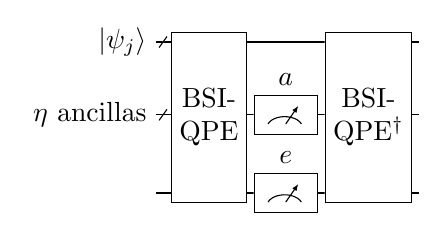
\begin{tikzpicture}
\begin{yquant*}
% init {$\eta$ ancillas} (a);
qubit {$\ket{\psi_j}$} system;
qubit {$\eta$ ancillas} a;
qubit {} f;

slash system;
slash a;
hspace {0.1cm} -;

box {BSI-\\QPE} (a,system,f);

["$a$",type=qubit]
measure a;

["$e$",type=qubit]
measure f;

box {BSI-\\QPE$^{\dagger}$} (a,system,f);
\end{yquant*}
\end{tikzpicture}

\caption{Quantum circuit for implementing projective measurement $E_{ae}$. }
\label{fig:Ecircuit}
\end{figure}
The dimensionless phase index obeys $(-1)^ea\equiv 2^\eta E_jt/(2\pi)\pmod{2^\eta}$ within the resolution window. Thus a physical energy representative is $\widetilde E_{a,e}=(2\pi/(2^\eta t))(-1)^ea$, with the branch chosen modulo $2\pi/t$. It is important to note that the measurement does not return the ancillas to a completely disentangled state. All $\eta+1$ phase-estimation ancillas (the $\eta$-qubit register and the sign/window qubit) must begin each full update process in the $\ket{0}$ state.
\subsection{Update}
\label{section:update}
After measuring the initial energy we must apply an update to our state. In quantum metropolis this update comes in the form of a unitary operator $C$ chosen from some set $\mathcal{C}$ according to some probability measure $d\mu(C)$. It is essential for the purposes of detailed balance that the probability of choosing $C \in \mathcal{C}$ is equal to the probability of choosing $C^{\dagger} \in \mathcal{C}$ (which is alternatively expressed as $d\mu(C) = d\mu(C^{\dagger})$).
\subsection{Accept or Reject}
\label{section:acceptprob}
After applying our unitary update $C$ we must decide whether to accept or reject this update. To ensure the probability of acceptance is approximately $\tilde{f}_{E_aE_b}$, we use a combination of phase estimation, controlled rotations and single qubit measurement (illustrated in Fig~\ref{fig:Qcircuit}). First we use phase estimation to prepare an ancilla register with an approximation $b$ to the new energy $E_b$:
\begin{equation}
   \frac{1}{\sqrt{2^{\eta}}}\sum_{j,b,p}G_j^{bp}\otimes\ket{b}\bra{p}\otimes\ket{\psi_j}\bra{\psi_j}
\end{equation}
Then using the known initial energy estimate $a$ we perform a $W_{a}$ rotation upon an ancilla qubit (initialised to $\ket{0}$ at the beginning of the update process) controlled by the ancilla register (and conditioned on the measurement result $e$ from $E_{ae}$):
\begin{equation}
    W_{abde} = \begin{pmatrix}
        \sqrt{1 - f_{abde}} & \sqrt{f_{abde}}\\
       \sqrt{f_{abde}} & -\sqrt{1 - f_{abde}}
    \end{pmatrix}
\end{equation}
Therefore, upon measuring this ancilla qubit the probability of measuring $s=1$ is given by $f_{abde}$ which we choose such that it is approximately $\tilde f_{E_aE_b}$. This is insufficient to prove that quantum metropolis converges to a gibbs state, however it does highlight the similarities with classical metropolis. In Section~\ref{section:why} we will prove the convergence rigorously.

If we measure $s=0$ (reject), then we proceed by applying $W_{a}^{\dagger}$ ($=W_a$) again after the measurement before applying inverse phase estimation and $C^{\dagger}$, to make the whole sequence ($Q_s^{ae}$) a projective binary measurement:
\begin{multline}
    Q_s^{ae} = \frac{1}{2^{\eta}}\sum_{j,p,q,b,d}
    C^{\dagger}\ket{\psi_j}\bra{\psi_j}C \otimes \ket{q}\bra{p}\\
    {}\otimes G_j^{bq\dagger}\ket{d}\bra{d}G_j^{bp}\otimes R^{abde}_s
\end{multline}
where $R^{abde}_s = W_{abde}\ket{s}\bra{s}W_{abde}$. If instead we measure $s=1$ (accept) we simply measure the energy register and then apply inverse BSI-QPE. We represent this accept process as $L^a_b$ as defined in Fig.~\ref{fig:LQ_circuit} and gives the following operator:
\begin{multline}
    L^{ade}_b = \frac{1}{2^{\eta}}\sum_{j,p,q}
    \ket{\psi_j}\bra{\psi_j}C \otimes \ket{q}\bra{p}\\
    {}\otimes G^{bq\dagger}_j \ket{d}\bra{d}G^{bp}_j
    \otimes \ket{1}\bra{1}W_{abde}
\end{multline}

It is crucial that the $\eta+2$ ancillas used in this first $Q^a_s$ measurement are different to those used in the $E_a$ measurement, and begin initialized to $\ket{0}$ at the beginning of each update process. However, it is equally important that every subsequent $Q_s^a$ measurement within the same update process reuses the ancillas without resetting them. This is highlighted by Fig.~\ref{fig:fullcircuit}. If instead ancillas were reset between measurements, then the Marriott and Watrous rewinding argument presented below is invalidated.
\begin{figure}
\begin{tikzpicture}
\begin{yquant*}
% init {$\eta$ ancillas} (a);
qubit {$\ket{\psi_j}$} system;
qubit {$\eta+1$ ancillas} a;
qubit {ancilla} f;

slash system;
slash a;
hspace {0.1cm} -;
box {$C$} (system);
box {BSI-\\QPE} (a,system);
[multictrl]
box {$W_{abde}$} (f) ~ a;



["$s$",type=qubit]
measure f;
% text {$\ket{b}$} (a);


[multictrl]
box {$W_{abde}$} (f) ~ a;

box {BSI-\\QPE$^{\dagger}$} (a,system);
box {$C^{\dagger}$} (system);
\end{yquant*}
\end{tikzpicture}

\caption{Quantum circuit for implementing projective measurement $Q_s^{ae}$. The same measurement ancilla is reused in every $Q_s^{ae}$ in an update step without being reset. It is necessary to apply $W_{abde}$ before and after the measurement to make the whole measurement projective (as $W_{abde}^{\dagger} = W_{abde}$). The slashed control is used to denote multiplexed control \cite{low2024trading}.}
\label{fig:Qcircuit}
\end{figure}

\begin{figure}
\begin{tikzpicture}
\begin{yquant*}
% init {$\eta$ ancillas} (a);
qubit {$\ket{\psi_j}$} system;
qubit {$\eta+1$ ancillas} a;
qubit {ancilla $\ket{0}$} f;

slash system;
slash a;
hspace {0.1cm} -;
box {$C$} (system);
box {BSI-\\QPE} (a,system);
[multictrl]
box {$W_{abde}$} (f) ~ a;



["$s=1$",type=qubit]
measure f;
["$b\>\>d$",type=qubit]
measure a;
% text {$\ket{b}\bra{b}$} (a);
box {BSI-\\QPE$^{\dagger}$} (a,system);
\end{yquant*}
\end{tikzpicture}

\caption{Quantum circuit for implementing accept process $L_b^a$.}
\label{fig:LQ_circuit}
\end{figure}
\subsection{Rejection process}
Upon rejection in the classical algorithm we can simply revert back to an earlier copy we made of the initial state or we may be able to reverse the update applied. However, in the quantum setting the no-cloning principle rules out the former and the irreversibility of measurement rules out the latter. Therefore, we need a new technique to return to our initial state.

We use an iterative sequence of binary projective measurements similar to the QMA verification amplification of Marriott and Watrous \cite{MarriottWatrous}. The first measurement $Q_s^{ae}$ has already been introduced, whilst the second $P_s^{ae}$ simply reports whether the state has returned to the initial energy:


\begin{equation}
    P^{ae}_1 = \frac{1}{2^{\eta}}\sum_{j,p,q} \left( \ket{\psi_j}\bra{\psi_j} \otimes \ket{q}\bra{p} \otimes G_j^{aq\dagger}\ket{e}\bra{e}G_j^{ap} \right)
\end{equation}
\begin{multline}
    P^{ae}_0 = \frac{1}{2^{\eta}}\sum_{j,p,q} \sum_{b}\bigg( \ket{\psi_j}\bra{\psi_j} \otimes \ket{q}\bra{p} \otimes \\G_j^{bq\dagger}(\mathbb{I} - \delta_{ab}\ket{e}\bra{e})G_j^{bp}  \bigg)
\end{multline}
This measurement is conducted as demonstrated by Fig~\ref{fig:Pcircuit}. It is crucial that the $\eta + 1$ ancillas used in $P_s^{ae}$ are the same as those used in $E_a$, and that the same ancillas are reused in every subsequent application of $P_s^{ae}$ as shown in Fig~\ref{fig:fullcircuit}.
\begin{figure}
\begin{tikzpicture}
\begin{yquant*}
% init {$\eta$ ancillas} (a);
qubit {$\ket{\psi_j}$} system;
qubit {$\eta+1$ ancillas} a;
qubit {$\ket{0}$} f;

slash system;
slash a;
hspace {0.1cm} -;
box {BSI-QPE} (a,system);

[multictrl]
box { $X$} f ~ a;

["$s$",type=qubit]
measure f;


box {BSI-QPE$^{\dagger}$} (a,system);
\end{yquant*}
\end{tikzpicture}

\caption{Quantum circuit for implementing projective measurement $P_s^{ae}$. The measurement ancilla introduced here does not need to be reused in each $P_s^{ae}$, unlike the measurement ancilla in $Q_s^{ae}$. The controlled $X$ gate is only triggered by the state $\ket{a}\ket{e}$ on the ancilla registers.}
\label{fig:Pcircuit}
\end{figure}
\begin{figure*}
    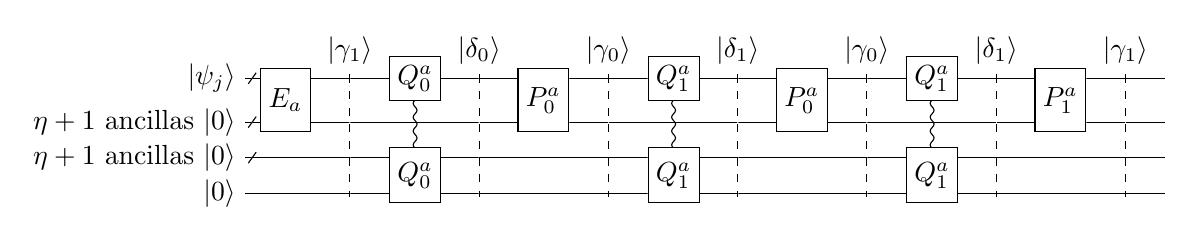
\begin{tikzpicture}
\begin{yquant*}
qubit {$\ket{\psi_j}$}  s;
qubit {$\eta +1$ ancillas $\ket{0}$} panc;
qubit {$\eta +1$ ancillas $\ket{0}$} qanc;
qubit {$\ket{0}$} m;
slash s;
slash qanc;
slash panc;
hspace {0.1cm} -;
box {$E_a$} (s,panc);
["$\ket{\gamma_1}$"]
barrier (-);
box {$Q^a_0$} (s,qanc, m);
["$\ket{\delta_0}$"]
barrier (-);
box {$P^a_0$} (s,panc);
["$\ket{\gamma_0}$"]
barrier (-);
box {$Q^a_1$} (s,qanc, m);
["$\ket{\delta_1}$"]
barrier (-);
box {$P^a_0$} (s,panc);
["$\ket{\gamma_0}$"]
barrier (-);
box {$Q^a_1$} (s,qanc, m);
["$\ket{\delta_1}$"]
barrier (-);
box {$P^a_1$} (s,panc);
["$\ket{\gamma_1}$"]
barrier (-);
\end{yquant*}
\end{tikzpicture}
\caption{Successfully completed rejection procedure demonstrating how the ancilla qubits used for $Q_s^{ae}$ are only reused by $Q_s^{ae}$ and the same for $P_s^{ae}$. This circuit corresponds to a term in $\mathcal{B}(2)[\rho]$ for $\{s_n\} = \{1,1\}$ and, within a single invariant subspace $\lambda$ (see Section~\ref{section:rejection}), occurs with probability $(1-p^{ae\lambda})^4(p^{ae\lambda})^2$. The state labels at the barriers denote the corresponding states of each invariant subspace.}
\label{fig:fullcircuit}
\end{figure*}

The iterative process proceeds as follows after measuring $s=0$ (reject) from the initial $Q_s^{ae}$ measurement: 
\begin{enumerate}
    \item Measure $P_s^{ae}$
        \begin{enumerate}
            \item If $s=1$ \textbf{terminate} as the state has returned to the approximate energy of the initial state.
            \item If $s=0$ continue.
        \end{enumerate}
    \item Measure $Q_s^a$
    \item Repeat up to a maximum of $n^*$ iterations
\end{enumerate}
% Each repetition has a constant chance of success as shown below and hence the iterative process has an exponentially small probability of failing to correctly reject the update, as we will now demonstrate using techniques originating in \cite{MarriottWatrous}. 

Let us consider the action of the rejection process on each eigenvector $\ket{\psi_j}$ of $H$. After measuring the energy $a$ at the beginning of the metropolis step we are left with post-measurement state $\frac{E_{ae}\ket{\psi_j}\ket{0}}{\|E_{ae} \ket{\psi_j}\ket{0}\|}$. We can see that this state must be a $+1$ eigenstate of the projector $P^{ae}_1$ due to the relation $P_1^{ae}E_{ae} = E_{ae}$.  Furthermore, as $P_1^{ae}$ commutes with $P^{ae}_1Q^{ae}_0P^{ae}_1$ they must be jointly diagnosable. Therefore our post measurement state can be written as a sum of joint eigenstates $\ket{\gamma_1^{a \lambda}}$ of $P^{ae}_1Q^{ae}_0P^{ae}_1$ and $P_1^{ae}$:
\begin{equation}
    \frac{E_{ae}\ket{\psi_j}\ket{0}}{\|E_{ae} \ket{\psi_j}\ket{0}\|} = \sum_{\lambda} c_{\lambda}^{aej}\ket{\gamma_1^{ae \lambda}}
\end{equation}
Writing the eigenvalue of $\ket{\gamma^{ae\lambda}_1}$ as $1-p^{ae\lambda}$, we have: \begin{align}1-p^{ae\lambda}&=\bra{\gamma^{ae\lambda}_1}P^{ae}_1Q^{ae}_0P^{ae}_1\ket{\gamma^{ae\lambda}_1} \\&=\|Q^{ae}_0P^{ae}_1\ket{\gamma^{ae\lambda}_1}\|^2\\ &= 1-\|Q^{ae}_1\ket{\gamma^{ae\lambda}_1}\|^2
\end{align}
so $p^{ae\lambda} = \|Q^{ae}_1\ket{\gamma^{ae\lambda}_1}\|^2$, and the probability of accepting the update is given by the mixture $p_{aej} = \sum_{\lambda}|c^{aej}_{\lambda}|^2p^{ae\lambda}$. Therefore, for each $\lambda$ with $p^{ae\lambda} \in (0,1)$ we can define the following 2D invariant subspace (we have suppressed the $ae\lambda$ labels for the remainder of this section for clarity, writing $\ket{\gamma_1} = \ket{\gamma^{ae\lambda}_1}$ and $p = p^{ae\lambda}$):
\begin{align}
    \ket{\delta_0} &= \frac{Q^{ae}_0P^{ae}_1\ket{\gamma_1}}{\sqrt{1-p}} &\ket{\delta_1} &= \frac{Q^{ae}_1P^{ae}_1\ket{\gamma_1}}{\sqrt{p}} \\
    \ket{\gamma_0} &= \frac{P^{ae}_0Q^{ae}_0\ket{\delta_0}}{\sqrt{p}} &\ket{\gamma_1} &= \frac{P^{ae}_1Q^{ae}_0\ket{\delta_0}}{\sqrt{1-p}}
\end{align}
From these definitions the following relations can be deduced:
\begin{align}
\begin{split}
\label{eq:deltagamma0}
    P^{ae}_1 \ket{\gamma_1} &= (Q^{ae}_0+Q^{ae}_1)P^{ae}_1 \ket{\gamma_1}\\
    &= Q^{ae}_0P^{ae}_1 \ket{\gamma_1}+Q^{ae}_1P^{ae}_1 \ket{\gamma_1}\\
    &= \sqrt{1-p} \ket{\delta_0} + \sqrt{p}\ket{\delta_1}\\
    Q^{ae}_0\ket{\delta_0} &= \sqrt{p} \ket{\gamma_0} + \sqrt{1-p} \ket{\gamma_1}
\end{split}
\end{align}
As $P^{ae}_1 \ket{\gamma_1} = \ket{\gamma_1}$ and $Q^{ae}_0\ket{\delta_0} = \ket{\delta_0}$ we can simplify the above and then through substitution deduce the remaining relations:
\begin{align}
\begin{split}
\label{eq:deltagamma1}
        \ket{\delta_1} &= -\sqrt{1-p} \ket{\gamma_0} + \sqrt{p} \ket{\gamma_1}\\
    \ket{\gamma_0} &= \sqrt{p} \ket{\delta_0} - \sqrt{1-p}\ket{\delta_1}
\end{split}
\end{align}
Therefore it is clear that each measurement transitions the state from one of $\ket{\delta_i}$ to one of $\ket{\gamma_i}$ or vice versa, whilst remaining within the same 2D invariant subspace. As the subspaces corresponding to different $\lambda$ are mutually orthogonal (which follows from the orthogonality of the $\ket{\gamma^{ae\lambda}_1}$ together with the relations above) and each is preserved by both measurements, the subspaces do not mix at any point during the rejection process. The probability of these transitions are trivially deduced from \eqref{eq:deltagamma0} and \eqref{eq:deltagamma1}, and can be seen in Fig.~\ref{fig:transitions}.
\begin{figure}
    \centering
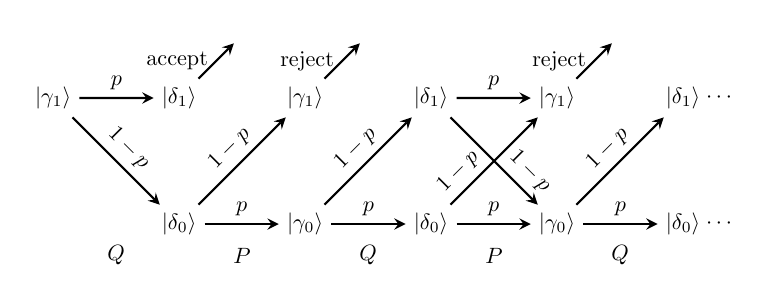
\begin{tikzpicture}[node distance=2cm, >=stealth, thick, scale=0.8, transform shape]
    \node (g-1t) at (0,2) {$|\gamma_1\rangle$};
    \node (s0t)  at (2,2) {$|\delta_1\rangle$};
    \node (s0)  at (2,0) {$|\delta_0\rangle$};
    \node (g0)  at (4,0) {$|\gamma_0\rangle$};
    \node (s1)  at (6,0) {$|\delta_0\rangle$};
    \node (g1)  at (8,0) {$|\gamma_0\rangle$};
    \node (s2)  at (10,0) {$|\delta_0\rangle$};
    \node (...1) at (10.6,0) {$\cdots$};
    \node (...2) at (10.6,2) {$\cdots$};
    
    \node (a) at (3,3) {};
    \node (r1) at (5,3) {};
    \node (r2) at (9,3) {};
    
    \node (g1t) at (4,2) {$|\gamma_1\rangle$};
    \node (s1t) at (6,2) {$|\delta_1\rangle$};
    \node (g2t) at (8,2) {$|\gamma_1\rangle$};
    \node (s2t) at (10,2) {$|\delta_1\rangle$};
    
    % Transitions
    \draw[->] (s0) -- node[above] {$p$} (g0);
    \draw[->] (g0) -- node[above] {$p$} (s1);
    \draw[->] (s1) -- node[above] {$p$} (g1);
    \draw[->] (g1) -- node[above] {$p$} (s2);
    
    \draw[->] (s0) -- node[above,sloped] {$1-p$} (g1t);
    \draw[->] (g0) -- node[above ,sloped] {$1-p$} (s1t);
    \draw[->] (s1) -- node[above left,sloped] {$1-p$} (g2t);
    \draw[->] (s1t) -- node[above] {$p$} (g2t);
    \draw[->] (g-1t) -- node[above] {$p$} (s0t);
    
    \draw[->] (s1t) -- node[above right,sloped] {$1-p$} (g1);
    \draw[->] (g1) -- node[above ,sloped] {$1-p$} (s2t);
    \draw[->] (g-1t) -- node[above ,sloped] {$1-p$} (s0);

    \draw[->] (s0t) -- node[left] {accept} (a);
    \draw[->] (g1t) -- node[left] {reject} (r1);
    \draw[->] (g2t) -- node[left] {reject} (r2);

    % Labels
    \node at (1,-0.5) {$Q$};
    \node at (3,-0.5) {$P$};
    \node at (5,-0.5) {$Q$};
    \node at (7,-0.5) {$P$};
    \node at (9,-0.5) {$Q$};
\end{tikzpicture}
    \caption{Markov chain showing the transition probability between the 4 states of a single invariant subspace $\lambda$ (with $p = p^{ae\lambda}$) upon each projective measurement. The full rejection process is a mixture of such chains weighted by $|c^{aej}_{\lambda}|^2$.}
    \label{fig:transitions}
\end{figure}

Take $n^*\geq1$ to be the number of complete $Q$--$P$ rounds allowed after the initial rejected $Q$ outcome and first failed $P$ test. The endpoint sectors $p=0,1$ contribute zero failure probability. For $p\in(0,1)$, the probability of attempting to reject and then failing the rejection process is $p(1-p)(p^2 +(1-p)^2)^{n^*}$. As the subspaces do not mix, the fixed-input failure probability $p_{aej}^{\mathrm{fail}}$ is the corresponding mixture over subspaces (reinstating the suppressed labels):
\begin{equation}
   p_{aej}^{\mathrm{fail}} =  \sum_{\lambda}|c^{aej}_{\lambda}|^2p^{ae\lambda}(1-p^{ae\lambda})((p^{ae\lambda})^2 +(1-p^{ae\lambda})^2)^{n^*}
\end{equation}
For all $p \in [0,1]$ we have: 
\begin{equation}
    p(1-p)(p^2 +(1-p)^2)^{n^*} \leq \frac{1}{2(n^*+1)} \left(\frac{n^*}{n^*+1}\right)^{n^*}
\end{equation}
Therefore, as $\sum_{\lambda}|c^{aej}_{\lambda}|^2=1$ we have:
\begin{equation}
    \label{eq:probabilty_of_rejection}
   p_{aej}^{\mathrm{fail}} \leq \frac{1}{2(n^*+1)} \left(\frac{n^*}{n^*+1}\right)^{n^*} \leq \frac{1}{2n^*}
\end{equation}
If the rejection process fails then the whole algorithm fails irrecoverably and must be restarted from the original initial state.

% We can evaluate $p_{aj}$ exactly as:
% \begin{equation}
%     p_{aj} = \sum_{\substack{b,k,\\p,q}} f_{ab}\alpha^{aq}_j \alpha_j^{ap} \alpha_k^{bp} \alpha_k^{bq} \| \bra{\psi_j} C \ket{\psi_k}\|^2
%     \label{eq:paj_exact}
% \end{equation}
\label{section:rejection}

\section{Why it works}
\label{section:why}
The classical Metropolis-Hastings algorithm works by constructing a Markov Chain through proposing and accepting/rejecting moves with probabilities determined by the energy difference between the initial and modified states. The transition matrix of this Markov chain is in detailed balance with respect to the Gibbs state, implying that the Gibbs state is a fixed point of the Markov chain. As Markov chain is also ergodic, it is known that it must have a single unique fixed point and converge towards it. Therefore, the Markov chain converges to the Gibbs state.

In the quantum metropolis algorithm we similarly construct a quantum Markov chain by proposing and accepting/rejecting moves based upon energy differences. However, as the energy differences cannot be resolved exactly we cannot prove exact detailed balance and must propose an alternative notion of approximate quantum detailed balance. A number of different definitions of approximate quantum detailed balance are already present in the literature \cite{}, however, we must go beyond these to incorporate additive errors to fully account for the non-zero (but exponentially suppressed) tails of BSI-QPE. By showing that the CP map that characterises the quantum Markov chain is in approximate quantum detailed balance with respect to the Gibbs state we know that the fixed point of the quantum Markov chain is very close to the Gibbs state. Further, we can ensure the quantum Markov chain is ergodic by choosing our update set $\{C\}$ to be a universal gate set \cite{Temme_2011} and hence that the quantum Markov chain converges to the fixed point close to the Gibbs state.

Below we present our modified formulation of approximate quantum detailed balance:

For any completely positive map $\mathcal{M}$ ($\mathcal{M}[\rho] =\sum_{j}  A_{j}\rho  A^{\dagger}_{j}$) and density matrix $\sigma$, we define $\mathcal{M}_{\sigma}[\rho] =\sum_{j}  A_{j}\sigma^{\frac{1}{2}}\rho\sigma^{\frac{1}{2}}  A^{\dagger}_{j}$ and $ \mathcal{M}^*_{\sigma}[\rho] = \sum_{j} \sigma^{\frac{1}{2}}A^{\dagger}_{j}\rho A_{j}\sigma^{\frac{1}{2}}$.
\begin{lemma}
\label{lemma:1}
Given a completely positive map $\mathcal{M}$ on $d$-dimensional density matrices and a density matrix $\sigma$, suppose that for every density matrix $\rho$ and every operator $X$ with $\|X\|\leq1$,
\begin{equation}
    \operatorname{Tr}\left[X \mathcal{M}^*_{\sigma}[\rho]\right] = \operatorname{Tr}\left[X\mathcal{M}_{\sigma}[\rho]\right](1+\epsilon^{X,\rho}_m) + \epsilon^{X,\rho}_a
    \label{eq:approximate_quantum_detailed_balance_condition}
\end{equation}
where $|\epsilon^{X,\rho}_m| \leq \epsilon_m$ and $|\epsilon^{X,\rho}_a| \leq \epsilon_a$. Then
 \begin{equation}
    \|\mathcal{M}^*_{\sigma}[\mathbb{I}]-\mathcal{M}[\sigma] \|_* \leq \|\mathcal{M}[\sigma]\|_*\epsilon_m + d\epsilon_a
    \label{eq:trace_detailed_balance_condition}
\end{equation}
where $\|\cdot\|_*$ is the trace norm and $\|\cdot\|$ is the operator norm. More generally, for any two linear maps $\mathcal{M}$ and $\mathcal{N}$ with $\|\mathcal{N}-\mathcal{M}\|_{\diamond}\leq\delta$,
\begin{equation*}
    \|\mathcal{N}^*_{\sigma}[\mathbb{I}]-\mathcal{N}[\sigma]\|_*
    \leq \|\mathcal{M}^*_{\sigma}[\mathbb{I}]-\mathcal{M}[\sigma]\|_*+2\delta.
\end{equation*}
Consequently the first bound may be substituted on the right whenever
$\mathcal M$ obeys the scalar premise above.
\end{lemma}

\begin{proof}
    If \eqref{eq:approximate_quantum_detailed_balance_condition} holds then for $\rho = \frac{\mathbb{I}}{d}$:
    \begin{equation}
        \operatorname{Tr}\left[X (\mathcal{M}^*_{\sigma}[\mathbb{I}]-\mathcal{M}_{\sigma}[\mathbb{I}])\right] = \operatorname{Tr}\left[X\mathcal{M}_{\sigma}[\mathbb{I}]\right]\epsilon^{X,\mathbb{I}/d}_m + d\epsilon^{X,\mathbb{I}/d}_a
    \end{equation}
    Further, by definition:
    \begin{equation}
        \mathcal{M}_{\sigma}[\mathbb{I}] = \mathcal{M}[\sigma]
    \end{equation}
    Therefore,
    \begin{equation}
    \label{eq:lhs}
        \left|\operatorname{Tr}\left[X
        (\mathcal{M}^*_{\sigma}[\mathbb{I}]-\mathcal{M}[\sigma])\right]\right|
        \leq \epsilon_m\left|\operatorname{Tr}\left[X\mathcal{M}[\sigma]\right]\right|
        +d\epsilon_a
    \end{equation}
    By the H\"older inequality for Schatten norms we can see that: 
        \begin{equation}
        |\operatorname{Tr}[X\mathcal{M}[\sigma]]| \leq \|X\|\|\mathcal{M}[\sigma]\|_*
    \end{equation}
    By taking the SVD of $(\mathcal{M}^*_{\sigma}[\mathbb{I}]-\mathcal{M}[\sigma]) = U\Sigma V^{\dagger}$ and choosing $X = VU^{\dagger}$, we obtain the claimed trace-norm bound. For the stability statement, set $\Delta=\mathcal{N}-\mathcal{M}$. The definition and dual characterization of the diamond norm give
    \begin{align*}
        \|\Delta[\sigma]\|_* &\leq \delta,\\
        \|\sigma^{1/2}\Delta^*[\mathbb{I}]\sigma^{1/2}\|_*
        &=\max_{\|X\|\leq1}\left|\operatorname{Tr}\left[\Delta(\sigma^{1/2}X\sigma^{1/2})\right]\right|\leq\delta,
    \end{align*}
    since $\|\sigma^{1/2}X\sigma^{1/2}\|_*\leq1$. The triangle inequality then yields
    \begin{equation}
        \|\mathcal{N}^*_{\sigma}[\mathbb{I}]-\mathcal{N}[\sigma]\|_*
        \leq \|\mathcal{M}^*_{\sigma}[\mathbb{I}]-\mathcal{M}[\sigma]\|_*+2\delta,
    \end{equation}
    which completes the proof.
\end{proof}
\begin{theorem}[Component Trace-Defect Bound]
\label{theorem:quantumapproximatedeatildedbalance}
Let $\mathcal{E}$ be a completely positive trace-preserving map, decomposed into completely positive maps indexed by the disjoint sets $G$ and $R$:
\begin{equation}
    \mathcal{E}[\rho] = \sum_{j\in G}\mathcal{M}_j[\rho]+\sum_{j\in R}\mathcal{M}_j[\rho].
\end{equation}
For a density matrix $\sigma$, suppose that every map indexed by $G$ obeys the trace-norm condition in Eq.~\eqref{eq:trace_detailed_balance_condition}, in the direct form
\begin{equation}
    \|\mathcal{M}_{j,\sigma}^*[\mathbb{I}]-\mathcal{M}_j[\sigma]\|_*\leq\delta_j,
    \qquad j\in G.
\end{equation}
No detailed-balance condition is required for the maps indexed by $R$. Then
\begin{multline}
     \|\mathcal{E}[\sigma]-\sigma\|_* \leq
     \sum_{j\in G}\min\left(\delta_j,2\|\mathcal{M}_j[\sigma]\|_*\right)\\
     +2\sum_{j\in R}\|\mathcal{M}_j[\sigma]\|_*.
\end{multline}
\end{theorem}
\begin{proof}
    By the triangle inequality we have:
    \begin{equation}
        \|\mathcal{E}^*_{\sigma}[\mathbb{I}]-\mathcal{E}[\sigma]\|_* \leq \sum_j \|\mathcal{M}^*_{j,\sigma}[\mathbb{I}]-\mathcal{M}_{j}[\sigma]\|_*
    \end{equation}
    As $\mathcal{E}$ is trace-preserving, we know that:
    \begin{equation}
        \mathcal{E}^*_{\sigma}[\mathbb{I}] = \sum_{j} \sigma^{\frac{1}{2}}A^{\dagger}_{j} A_{j}\sigma^{\frac{1}{2}} = \sigma
    \end{equation}
    Therefore,
    \begin{equation}
        \|\sigma - \mathcal{E}[\sigma]\|_* \leq \sum_j \|\mathcal{M}^*_{j,\sigma}[\mathbb{I}]-\mathcal{M}_{j}[\sigma]\|_*
    \end{equation}
    Further, as both
$\mathcal{M}_{j,\sigma}^{*}[\mathbb{I}]$ and
$\mathcal{M}_j[\sigma]$ are positive semidefinite:
    \begin{align}
        \|\mathcal{M}^*_{j,\sigma}[\mathbb{I}]\|_* &= \operatorname{Tr}\left[\sum_l \sigma^{\frac{1}{2}} K_{jl}^{\dagger} K_{jl} \sigma^{\frac{1}{2}}\right]\\
        &= \operatorname{Tr}\left[\sum_l K_{jl}\sigma K_{jl}^{\dagger}\right]\\
        &= \|\mathcal{M}_{j}[\sigma]\|_*
    \end{align}
    Therefore,
    \begin{equation}
         \|\mathcal{M}^*_{j,\sigma}[\mathbb{I}]-\mathcal{M}_{j}[\sigma]\|_* \leq 2\|\mathcal{M}_{j}[\sigma]\|_*
    \end{equation}
    Hence,
    \begin{multline}
        \|\sigma-\mathcal{E}[\sigma]\|_* \leq
        \sum_{j\in G}\min\left(\delta_j,2\|\mathcal{M}_j[\sigma]\|_*\right)\\
        +2\sum_{j\in R}\|\mathcal{M}_j[\sigma]\|_*.
    \end{multline}
\end{proof}
\begin{lemma}[Reduced-Kraus reversal bound]
\label{lemma:reduced_kraus_reversal}
Let $\mathcal M[\rho]=\int_\Omega K_\omega\rho K_\omega^\dagger\,d\omega$
be completely positive, let $\sigma$ be a density operator, and let
$\vartheta:\Omega\to\Omega$ be a measure-preserving involution.  Suppose
that, for some $a\geq0$,
\begin{equation}
 \left\|K_\omega\sqrt\sigma-\sqrt\sigma K_{\vartheta\omega}^\dagger\right\|_2
 \leq a\left\|K_\omega\sqrt\sigma\right\|_2
 \quad\text{for almost every }\omega .
 \label{eq:reduced_kraus_reversal}
\end{equation}
Then, with $p_{\mathcal M}=\operatorname{Tr}\mathcal M[\sigma]$,
\begin{equation}
 \left\|\mathcal M_\sigma^*[\mathbb I]-\mathcal M[\sigma]\right\|_*
 \leq2a p_{\mathcal M}.
 \label{eq:reversal_defect}
\end{equation}
For a circuit operator $V_\omega$ acting on the system and an ancilla that
starts in $\ket0$, Eq.~\eqref{eq:reduced_kraus_reversal} is a condition on
the \emph{reduced} Kraus operators
$K_{\omega,z}=\langle z|V_\omega|0\rangle$; Hermiticity of $V_\omega$ on the
joint space alone is not sufficient.
\end{lemma}
\begin{proof}
Form Hilbert--Schmidt block columns $F=(K_\omega\sqrt\sigma)_\omega$ and
$G=(\sqrt\sigma K_{\vartheta\omega}^\dagger)_\omega$.  Measure preservation
and trace cyclicity give
\begin{align*}
 FF^\dagger&=\mathcal M[\sigma],&
 GG^\dagger&=\mathcal M_\sigma^*[\mathbb I],\\
 \|F\|_2^2&=\|G\|_2^2=p_{\mathcal M}.&&
\end{align*}
Equation~\eqref{eq:reduced_kraus_reversal} gives
$\|F-G\|_2\leq a\sqrt{p_{\mathcal M}}$.  Hence
\begin{equation*}
 \|FF^\dagger-GG^\dagger\|_*
 \leq(\|F\|_2+\|G\|_2)\|F-G\|_2
 \leq2a p_{\mathcal M}.
\end{equation*}
\end{proof}
\emph{Why the reduced condition is needed.}
Energy support alone does not imply a small trace defect: for
$H=0$, $\sigma=\mathbb I/2$, and $K=\ket1\!\bra0$, the energy bandwidth is
zero but
$\|\sqrt\sigma K^\dagger K\sqrt\sigma-K\sigma K^\dagger\|_*=1$.
Likewise, Hermiticity before discarding a fixed pure ancilla can produce a
reset channel after the discard.  Thus the reduced-system identities above
cannot be replaced by a joint-space Hermiticity argument.
% \begin{theorem}[Approximate Quantum Detailed Balance]
% \label{theorem:quantumapproximatedeatildedbalance}
%     Given a completely positive trace preserving
% map $\mathcal{E}$ on $d$-dimensional density matrices and a density matrix $\sigma$. Let $\mathcal{E}[\rho] =\sum_{j}  A_{j}\rho  A^{\dagger}_{j}$, $\mathcal{E}_{\sigma}[\rho] =\sum_{j}  A_{j}\sigma^{\frac{1}{2}}\rho\sigma^{\frac{1}{2}}  A^{\dagger}_{j}$ and $ \mathcal{E}^*_{\sigma}[\rho] = \sum_{j} \sigma^{\frac{1}{2}}A^{\dagger}_{j}\rho A_{j}\sigma^{\frac{1}{2}}$. If for all density matrices $\rho$ and operators $X$ with operator norm 1, we have:
% \begin{equation}
%     Tr\left[X \mathcal{E}_{\sigma}[\rho]\right] = Tr\left[X\mathcal{E}^*_{\sigma}[\rho]\right](1+\epsilon^{\rho \Pi}_m) + \epsilon^{\rho \Pi}_a
%     \label{eq:approximate_quantum_detailed_balance_condition}
% \end{equation}
% where $|\epsilon^{\rho \Pi}_m| \leq \epsilon_m$, $|\epsilon^{\rho \Pi}_a| \leq \epsilon_a$, then $\mathcal{E}$ is said to obey Approximate Quantum Detailed Balance with respect to $\sigma$. Therefore,
%  \begin{equation}
%     \|\mathcal{E}[\sigma] - \sigma\|_* \leq \epsilon_m + d\epsilon_a
% \end{equation}
% where $\|\cdot\|_*$ is the trace norm.
% \end{theorem}
% \begin{proof}
%     If \eqref{eq:approximate_quantum_detailed_balance_condition} holds then for $\rho = \frac{\mathbb{I}}{d}$:
%     \begin{equation}
%         Tr\left[X (\mathcal{E}_{\sigma}[\mathbb{I}]-\mathcal{E}^*_{\sigma}[\mathbb{I}])\right] = Tr\left[X\mathcal{E}^*_{\sigma}[\mathbb{I}]\right]\epsilon^{X}_m + d\epsilon^{X}_a
%     \end{equation}
%     Further, by definition:
%     \begin{equation}
%         \mathcal{E}^*_{\sigma}[\mathbb{I}] = \sum_{j} \sigma^{\frac{1}{2}}A^{\dagger}_{j} A_{j}\sigma^{\frac{1}{2}} = \sigma
%     \end{equation}
%     \begin{equation}
%         \mathcal{E}_{\sigma}[\mathbb{I}] = \mathcal{E}[\sigma]
%     \end{equation}
%     Therefore,
%     \begin{equation}
%         Tr\left[X (\mathcal{E}[\sigma]-\sigma)\right] = Tr\left[X\sigma\right]\epsilon^{ X}_m + d\epsilon^{X}_a
%     \end{equation}
%     As $Tr\left[X\sigma\right] \leq 1$ and $\|A\|_* = \max_{\|X\|=1} |Tr(XA)|$ we have that:
%     \begin{equation}
%         \|\mathcal{E}[\sigma]-\sigma\|_* \leq \epsilon_m + d\epsilon_a
%     \end{equation}
% \end{proof}
%  \begin{corollary}[Ergodicity of the square modulus for random-unitary channels \cite{Burgarth_2013}]
%      A random-unitary channel $M = \sum_{i\in X}p_i \mathcal{U}_i$ , with $\mathcal{U}_i (\rho) = U_i \rho U^{\dagger}_i$ , is mixing if the group representation
% generated by the unitaries $\{U^{\dagger}_i U_j \}_{i,j\in X}$ is irreducible. 
%  \end{corollary}
\begin{widetext}
To demonstrate an update round $\mathcal{E}$ of the Quantum Metropolis algorithm is in approximate quantum detailed balance with respect to the Gibbs state $\sigma_G$, we must express it as a completely positive trace preserving map:
\begin{equation}
    \mathcal{E}[\rho] = \mathcal{A}[\rho] + \sum_{n=0}^{n^*} \mathcal{B}(n)[\rho] + \mathcal{C}[\rho]
\end{equation}
where $\mathcal{A}$ corresponding to acceptance, $\mathcal{B}(n)$ to successful rejection after $n$ iterations and $\mathcal{C}$ to failing to reject after $n^*$ iterations:
\begin{equation}
    \mathcal{A}[\rho] = \int  \operatorname{Tr}_{\mathrm{anc}}\bigg[\sum_{a,b,d,e}L_b^{ade} E_{ae} ( \rho\otimes \ket{0}\bra{0}) 
     E_{ae}L^{ade\dagger}_b\bigg]d\mu(C)
\end{equation}
\begin{equation}
    \mathcal{B}(n)[\rho] = \int \operatorname{Tr}_{\mathrm{anc}}\bigg[\sum_{a,e,\{s\}}P^{ae}_1Q^{ae}_{s_n}\ldots P^{ae}_0Q^{ae}_{s_1}P^{ae}_0Q^{ae}_0E_{ae} ( \rho\otimes \ket{0}\bra{0})E_{ae}Q^{ae}_0P^{ae}_0Q^{ae}_{s_1}P^{ae}_0\ldots Q^{ae}_{s_n}P^{ae}_1\bigg]d\mu(C)
\end{equation}
\begin{equation}
    \mathcal{C}[\rho] = \rho_0 \int \operatorname{Tr}\bigg[\sum_{a,e,\{s\}}P^{ae}_0Q^{ae}_{s_{n^*}}\ldots P^{ae}_0Q^{ae}_{s_1}P^{ae}_0Q^{ae}_0E_{ae} ( \rho\otimes \ket{0}\bra{0})E_{ae}Q^{ae}_0P^{ae}_0Q^{ae}_{s_1}P^{ae}_0\ldots Q^{ae}_{s_{n^*}}P^{ae}_0\bigg]d\mu(C) 
\end{equation}
where $\rho_0$ is the initial state the overall Metropolis algorithm was started from. 


To use Theorem~\ref{theorem:quantumapproximatedeatildedbalance}, we place $\mathcal{A}$ and the maps $\mathcal{B}(n)$ in the certified set $G$, and place $\mathcal{C}$ in the unrestricted set $R$. We first consider real, support-truncated approximations $\tilde{\mathcal{A}}$ and $\tilde{\mathcal{B}}(n)$ obtained by substituting $\tilde\alpha,\tilde\beta$ for $\hat\alpha,\hat\beta$. Under this substitution $G^{pq}_j$ becomes the real matrix $\tilde G^{pq}_j$, whose entries vanish outside their bandwidth-$\mu$ support. We bound the trace defects of the tilde maps directly, in the form of Eq.~\eqref{eq:trace_detailed_balance_condition}, and transfer those bounds to the physical maps with the dimension-free diamond estimate in Lemma~\ref{lemma:1}. The scalar premise of Lemma~\ref{lemma:1} is therefore not required here. No detailed-balance condition is imposed on $\mathcal{C}$; Theorem~\ref{theorem:quantumapproximatedeatildedbalance} bounds it directly by its trace weight. We begin with $\tilde{\mathcal{A}}$.
    \begin{equation}
    Tr\left[X\tilde{\mathcal{A}}_{\sigma_G}[\rho]\right] = \int Tr\left[(X\otimes \mathbb{I})\sum_{a,b,d,e}\textcolor{blue}{\tilde L^{ade}_b} \textcolor{red}{\tilde E_{ae}} \sigma_G^{\frac{1}{2}} (\rho\otimes \ket{0}\bra{0}) \sigma_G^{\frac{1}{2}}\textcolor{red}{\tilde E_{ae}}\textcolor{blue}{\tilde L^{ade\dagger}_b}\right] d\mu(C)
\end{equation}
As $\sigma_G = \frac{1}{Z}\sum_j e^{-\beta E_j} \ket{\psi_j}\bra{\psi_j}$ where $\ket{\psi_j}$ are the eigenstates of $H$ with eigenvalues $E_j$. 
\begin{multline}
    Tr\left[X\tilde{\mathcal{A}}_{\sigma_G}[\rho]\right] =\frac{1}{2^{4\eta}Z} \sum_{jklmabde} e^{-\frac{\beta}{2}(E_j+E_k)}\textcolor{blue}{f_{abde}} \textcolor{blue}{\bra{\psi_l}}X\textcolor{blue}{\ket{\psi_m}}\textcolor{red}{\bra{\psi_j}}\rho\textcolor{red}{\ket{\psi_k}} \int \textcolor{blue}{\braket{\psi_m|C|\psi_j}\braket{\psi_k|C^{\dagger}|\psi_l}} d\mu(C)\\\sum_{p_1p_2} \textcolor{blue}{\bra{0} \tilde G^{b0\dagger}_l\ket{d}\bra{d}\tilde G^{bp_2}_l\tilde G^{bp_2\dagger}_m\ket{d}\bra{d}\tilde G^{b0}_m\ket{0}}
    \textcolor{red}{\bra{0}\tilde G_k^{a0\dagger}\ket{e}\bra{e}\tilde G_k^{ap_1}\tilde G_j^{ap_1\dagger}\ket{e}\bra{e}\tilde G_j^{a0}\ket{0}}
    \label{eq:Arho}
\end{multline}
Similarly,
\begin{multline}
    Tr\left[X\tilde{\mathcal{A}}^*_{\sigma_G}[\rho]\right] =\frac{1}{2^{4\eta}Z} \sum_{jklmabde} e^{-\frac{\beta}{2}(E_l+E_m)}\textcolor{blue}{f_{abde}} \textcolor{red}{\bra{\psi_l}}X\textcolor{red}{\ket{\psi_m}}\textcolor{blue}{\bra{\psi_j}}\rho\textcolor{blue}{\ket{\psi_k}} \int \textcolor{blue}{\braket{\psi_k|C|\psi_l}\braket{\psi_m|C^{\dagger}|\psi_j}} d\mu(C)\\\sum_{p_1p_2} \textcolor{blue}{\bra{0} \tilde G^{b0\dagger}_j\ket{d}\bra{d}\tilde G^{bp_2}_j\tilde G^{bp_2\dagger}_k\ket{d}\bra{d}\tilde G^{b0}_k\ket{0}}
    \textcolor{red}{\bra{0}\tilde G_m^{a0\dagger}\ket{e}\bra{e}\tilde G_m^{ap_1}\tilde G_l^{ap_1\dagger}\ket{e}\bra{e}\tilde G_l^{a0}\ket{0}}
        \label{eq:A*rho}  
\end{multline}
Due to the restricted support of $\tilde G^{pq}_j$ we can restrict the summations in Eq.~\eqref{eq:Arho} and Eq~\eqref{eq:A*rho} to $\chi$, where $\chi$ is the set of all $a,b,d,e$ such that all of the following conditions hold:
\begin{equation}
\begin{aligned}
    |a-(-1)^e\frac{2^{\eta}}{2\pi}E_lt|_{2^{\eta}} &\leq \mu  &|a-(-1)^e\frac{2^{\eta}}{2\pi}E_mt|_{2^{\eta}} &\leq \mu\\
    |b-(-1)^{d}\frac{2^{\eta}}{2\pi}E_jt|_{2^{\eta}} &\leq \mu   &|b-(-1)^{d}\frac{2^{\eta}}{2\pi}E_kt|_{2^{\eta}}& \leq \mu
\end{aligned}
\end{equation}
 We can relax these conditions to define $\chi' \supset \chi$  as all $a,b, d, e$ such that:
\begin{equation}
\label{eq:condJ}
        |(-1)^db-(-1)^ea -\frac{2^{\eta}t}{2\pi}(\frac{E_j+E_k-E_l-E_m}{2})|_{2^{\eta}} \leq 4\mu
\end{equation}
As $|E_j| \leq \|H\|$, if we choose $t = \frac{1}{16\|H\|}$ and $\mu < \frac{2^{\eta}}{64\pi}$ so that $E_j$ satisfies $-\frac{1}{8t} + 2\frac{2\pi}{2^{\eta}t}\mu < E_j < \frac{1}{8t} - 2\frac{2\pi}{2^{\eta}t}\mu$, then we have that $-2^{\eta-2}+4\mu < \frac{2^{\eta}t}{2\pi}(E_i -E_j) < 2^{\eta-2}-4\mu$ for all $i$ and $j$. Hence, within $\chi'$ the possible ranges of $(-1)^db-(-1)^ea$ are
\begin{multline}
    -2^{\eta+1}\leq(-1)^db-(-1)^ea<-7\cdot2^{\eta-2} \text{ or } -5\cdot2^{\eta-2}< (-1)^db-(-1)^ea < -3\cdot2^{\eta-2} \text{ or }-2^{\eta-2}< (-1)^db-(-1)^ea < 2^{\eta-2}\\ \text{ or } 3\cdot2^{\eta-2}< (-1)^db-(-1)^ea < 5\cdot2^{\eta-2}\text{ or } 7\cdot2^{\eta-2}< (-1)^db-(-1)^ea \leq 2^{\eta+1}
\end{multline}
By separately considering each of these regions we can rewrite condition~\eqref{eq:condJ} as the following:
\begin{equation}
    a,b,d,e \in \chi' \iff \begin{cases}
    |(-1)^db-(-1)^ea+2^{\eta+1}-\frac{2^{\eta}t}{2\pi}\frac{E_j+E_k-E_l-E_m}{2}|\leq 4\mu&\text{ for }-2^{\eta+1}\leq(-1)^db-(-1)^ea<-7\cdot2^{\eta-2}\\
    |(-1)^db-(-1)^ea+2^{\eta}-\frac{2^{\eta}t}{2\pi}\frac{E_j+E_k-E_l-E_m}{2}|\leq 4\mu&\text{ for }-5\cdot 2^{\eta-2}< (-1)^db-(-1)^ea < -3\cdot2^{\eta-2}\\
     |(-1)^db-(-1)^ea-\frac{2^{\eta}t}{2\pi}\frac{E_j+E_k-E_l-E_m}{2}|\leq 4\mu&\text{ for }-2^{\eta-2}< (-1)^db-(-1)^ea < 2^{\eta-2}\\
     |(-1)^db-(-1)^ea-2^{\eta}-\frac{2^{\eta}t}{2\pi}\frac{E_j+E_k-E_l-E_m}{2}|\leq 4\mu&\text{ for }3\cdot 2^{\eta-2}< (-1)^db-(-1)^ea < 5\cdot 2^{\eta-2}\\
     |(-1)^db-(-1)^ea-2^{\eta+1}-\frac{2^{\eta}t}{2\pi}\frac{E_j+E_k-E_l-E_m}{2}|\leq 4\mu&\text{ for }7\cdot2^{\eta-2}< (-1)^db-(-1)^ea \leq 2^{\eta+1}
    \end{cases}
    \label{eq:conditions}
\end{equation}
as $|x|_N = |x - kN| \text{ for } -\frac{N}{2} + kN \leq x \leq \frac{N}{2} + kN$.
Therefore, we chose $f_{abde}$ to be defined as:
\begin{equation}
    f_{abde} = \begin{cases}
    \min(1,e^{-\beta\frac{2\pi}{2^{\eta}t}((-1)^db-(-1)^ea+2^{\eta+1})})&\text{ for }-2^{\eta+1}\leq (-1)^db-(-1)^ea < -7\cdot2^{\eta-2}\\
    0&\text{ for }-7\cdot2^{\eta-2}\leq (-1)^db-(-1)^ea \leq -5\cdot2^{\eta-2}\\
    \min(1,e^{-\beta\frac{2\pi}{2^{\eta}t}((-1)^db-(-1)^ea+2^{\eta})})&\text{ for }-5\cdot 2^{\eta-2}< (-1)^db-(-1)^ea < -3\cdot2^{\eta-2}\\
    0&\text{ for }-3\cdot2^{\eta-2}\leq (-1)^db-(-1)^ea \leq -2^{\eta-2}\\
     \min(1,e^{-\beta\frac{2\pi}{2^{\eta}t}((-1)^db-(-1)^ea)})&\text{ for }-2^{\eta-2}<(-1)^db-(-1)^ea < 2^{\eta-2}\\
    0&\text{ for }2^{\eta-2}\leq (-1)^db-(-1)^ea \leq 3\cdot2^{\eta-2}\\
     \min(1,e^{-\beta\frac{2\pi}{2^{\eta}t}((-1)^db-(-1)^ea-2^{\eta})})&\text{ for }3\cdot 2^{\eta-2}< (-1)^db-(-1)^ea < 5\cdot2^{\eta-2}\\
     0&\text{ for }5\cdot2^{\eta-2}\leq (-1)^db-(-1)^ea \leq 7\cdot2^{\eta-2}\\
     \min(1,e^{-\beta\frac{2\pi}{2^{\eta}t}((-1)^db-(-1)^ea-2^{\eta+1})})&\text{ for }7\cdot 2^{\eta-2}< (-1)^db-(-1)^ea \leq 2^{\eta+1}
    \end{cases}
\end{equation}
so that $e^{-\frac{\beta}{2}(E_l+E_m)}f_{baed}$ for $b, a, e, d \in \chi'$ obeys:
\begin{equation}
    \begin{aligned}
    e^{-\frac{\beta}{2}(E_l+E_m)}f_{baed} &= e^{-\frac{\beta}{2}(E_l+E_m)}\min(1,e^{-\frac{\beta}{2}(E_j+E_k-E_l-E_m + 2\xi)})\\
    &= \min(e^{-\frac{\beta}{2}(E_l+E_m)}, e^{-\frac{\beta}{2}(E_j+E_k + 2\xi)})\\
    &= e^{-\frac{\beta}{2}(E_j+E_k + 2\xi)} \min(e^{-\frac{\beta}{2}(E_l+E_m-E_j-E_k-2\xi)},1)\\
    &= e^{-\frac{\beta}{2}(E_j+E_k + 2\xi)}f_{abde}\\
    &= e^{-\frac{\beta}{2}(E_j+E_k)}f_{abde}e^{-\beta\xi}
\end{aligned}
\label{eq:fabtofba}
\end{equation}
where $|\xi| \leq \frac{8\pi}{2^{\eta}t}\mu$. Since $\chi'\supset\chi$ and the summands vanish outside $\chi$, we may write the summation over $\chi'$:
\begin{multline}
   Tr\left[X\tilde{\mathcal{A}}^*_{\sigma_G}[\rho]\right] =\frac{1}{2^{4\eta}Z} \sum_{abde\in \chi'}\sum_{jklm} e^{-\frac{\beta}{2}(E_l+E_m)}f_{abde} \bra{\psi_l}X\ket{\psi_m}\bra{\psi_j}\rho\ket{\psi_k} \int \braket{\psi_k|C|\psi_l}\braket{\psi_m|C^{\dagger}|\psi_j} d\mu(C)\\\sum_{p_1p_2} \bra{0} \tilde G^{b0\dagger}_j\ket{d}\bra{d}\tilde G^{bp_2}_j\tilde G^{bp_2\dagger}_k\ket{d}\bra{d}\tilde G^{b0}_k\ket{0}
    \bra{0}\tilde G_m^{a0\dagger}\ket{e}\bra{e}\tilde G_m^{ap_1}\tilde G_l^{ap_1\dagger}\ket{e}\bra{e}\tilde G_l^{a0}\ket{0}
\end{multline}
By swapping the labels $a \leftrightarrow b$, $d \leftrightarrow e$, $p_1 \leftrightarrow p_2$ we get:
\begin{multline}
    Tr\left[X\tilde{\mathcal{A}}^*_{\sigma_G}[\rho]\right] =\frac{1}{2^{4\eta}Z} \sum_{abde\in \chi'}\sum_{jklm} e^{-\frac{\beta}{2}(E_l+E_m)}f_{baed} \bra{\psi_l}X\ket{\psi_m}\bra{\psi_j}\rho\ket{\psi_k} \int \braket{\psi_k|C|\psi_l}\braket{\psi_m|C^{\dagger}|\psi_j} d\mu(C)\\\sum_{p_1p_2} \bra{0} \tilde G^{a0\dagger}_j\ket{e}\bra{e}\tilde G^{ap_1}_j\tilde G^{ap_1\dagger}_k\ket{e}\bra{e}\tilde G^{a0}_k\ket{0}
    \bra{0}\tilde G_m^{b0\dagger}\ket{d}\bra{d}\tilde G_m^{bp_2}\tilde G_l^{bp_2\dagger}\ket{d}\bra{d}\tilde G_l^{b0}\ket{0}
\end{multline}
Equation~\eqref{eq:fabtofba} is an exact, termwise relation with
$e^{-\beta\xi}\in[e^{-\gamma_A},e^{\gamma_A}]$, where
\begin{equation}
 \gamma_A:=\frac{8\pi\beta\mu}{2^\eta t}.
 \label{eq:gamma_A}
\end{equation}
This factor cannot in general be pulled outside the complex sums above,
because those sums may contain cancellations.  The trace defect instead
follows from the reduced-Kraus pairing in
Lemma~\ref{lemma:reduced_kraus_reversal}.  For a complete acceptance history
$\omega=(C,a,b,d,e,z)$, define the reduced system Kraus operator
\begin{equation*}
 K^A_\omega:=\langle z|\tilde L_b^{ade}\tilde E_{ae}|0\rangle .
\end{equation*}
The required circuit-level reversal condition is the existence of a
measure-preserving involution
\begin{equation*}
 \vartheta_A(C,a,b,d,e,z)=(C^\dagger,b,a,e,d,z')
\end{equation*}
where the discrete relabelling $z\mapsto z'$ must reverse every retained
phase-register label and make $\vartheta_A^2$ the identity.  Together with
$d\mu(C)=d\mu(C^\dagger)$ this makes the involution measure preserving.
The condition is that
\begin{equation}
 \left\|K^A_\omega\sqrt{\sigma_G}
 -\sqrt{\sigma_G}(K^A_{\vartheta_A\omega})^\dagger\right\|_2
 \leq\left(e^{\gamma_A/2}-1\right)
 \left\|K^A_\omega\sqrt{\sigma_G}\right\|_2 .
 \label{eq:accept_reversal_condition}
\end{equation}
This reduced condition is stronger than the support relation
\eqref{eq:fabtofba}; it must be checked after taking the ancilla matrix
elements, rather than inferred from Hermiticity of the joint-space
projectors.  Whenever Eq.~\eqref{eq:accept_reversal_condition} holds,
Lemma~\ref{lemma:reduced_kraus_reversal} gives, with
$\tilde p_A:=\operatorname{Tr}\tilde{\mathcal A}[\sigma_G]$,
\begin{equation}
 \left\|\tilde{\mathcal A}_{\sigma_G}^*[\mathbb I]
 -\tilde{\mathcal A}[\sigma_G]\right\|_*
 \leq r_A\tilde p_A,\qquad
 r_A:=2\left(e^{\gamma_A/2}-1\right).
 \label{eq:accept_direct_defect}
\end{equation}
The update measure must also obey $d\mu(C)=d\mu(C^\dagger)$, as assumed in
Section~\ref{section:update}; at the level of matrix elements this gives
\begin{equation}
    \int  \bra{\psi_k}C\ket{\psi_{l}}\bra{\psi_m}C^{\dagger} \ket{\psi_j} d\mu(C) = \int  \bra{\psi_k}C^{\dagger}\ket{\psi_{l}}\bra{\psi_m}C \ket{\psi_j} d\mu(C)
\end{equation}

\begin{lemma}
\label{lemma:3}
Let $\{D_s\}_{s\in S}$ be mutually orthogonal projectors satisfying $\sum_{s\in S} D_s \leq \mathbb{I}$. Given a unitary $U$ define the projective measurement $K_s = U^{\dagger}D_s U$ and CP map $\mathcal{K}[\rho] = \sum_{s \in S} K_s\rho K_s^{\dagger}$. Further, given operator $\tilde U$, we define approximate measurements $\tilde K_s = \tilde U^{\dagger}D_s \tilde U$ and approximate map $\tilde{\mathcal{K}}[\rho] = \sum_{s \in S} \tilde K_s\rho \tilde K_s^{\dagger}$. If $\|U-\tilde U\| \leq \epsilon<1/4$ then
\begin{equation}
    \|\mathcal{K} - \tilde{\mathcal{K}}\|_{\diamond} \leq 6\epsilon
\end{equation}
\end{lemma}
\begin{proof}
Introduce a label register and the Stinespring block columns
\begin{equation*}
 V:=\sum_{s\in S}\ket{s}\otimes K_s,\qquad
 \tilde V:=\sum_{s\in S}\ket{s}\otimes\tilde K_s .
\end{equation*}
Then
$\mathcal K[\rho]=\operatorname{Tr}_{S}(V\rho V^\dagger)$ and likewise
for $\tilde{\mathcal K}$.  Expanding their difference and using
$\|\operatorname{Tr}_{S}(R_1\,\cdot\,R_2^\dagger)\|_\diamond
\leq\|R_1\|\|R_2\|$ gives
\begin{equation}
 \|\mathcal K-\tilde{\mathcal K}\|_\diamond
 \leq(\|V\|+\|\tilde V\|)\|V-\tilde V\|.
 \label{eq:stinespring_column_bound}
\end{equation}
Since the $D_s$ are mutually orthogonal and $U$ is unitary,
$V^\dagger V=\sum_sK_s\leq\mathbb I$, so $\|V\|\leq1$.  The same
orthogonality, together with $\|\tilde U\|\leq1+\epsilon$, gives
\begin{equation*}
 \|\tilde V\|\leq\|\tilde U\|^2\leq(1+\epsilon)^2.
\end{equation*}
Finally,
\begin{equation*}
 K_s-\tilde K_s
 =(U-\tilde U)^\dagger D_sU
 +\tilde U^\dagger D_s(U-\tilde U).
\end{equation*}
Stacking these differences in the label register and again using the
orthogonality of the $D_s$ gives
\begin{equation*}
 \|V-\tilde V\|\leq\epsilon+\epsilon(1+\epsilon)
 =\epsilon(2+\epsilon).
\end{equation*}
Substitution into Eq.~\eqref{eq:stinespring_column_bound} yields
\begin{equation*}
 \|\mathcal K-\tilde{\mathcal K}\|_\diamond
 \leq\epsilon(2+\epsilon)\bigl(1+(1+\epsilon)^2\bigr)
 \leq6\epsilon
\end{equation*}
for $\epsilon<1/4$.
\end{proof}
The maps
$\mathfrak{E}[\rho]=\sum_{a,e}E_{ae}\rho E_{ae}$,
$\mathcal P_S[\rho]=\sum_{s\in S}P_s\rho P_s$, and
$\mathcal Q_S[\rho]=\sum_{s\in S}Q_s\rho Q_s$ have the projective form
in Lemma~\ref{lemma:3}.  We postpone their measurements by storing the
outcomes in label registers; this is only a proof device.  By
Lemma~\ref{lemma:0}, substituting the real, support-truncated
$\tilde G_j^{pq}$ for $G_j^{pq}$ changes BSI-QPE by at most $u$.  Set
\begin{equation*}
 \lambda:=6u=6\frac{2\epsilon_\Delta+s_\mu\epsilon_r}{\sqrt{2^\eta}},
 \qquad u<\frac14 .
\end{equation*}
Lemma~\ref{lemma:3} therefore bounds the changes in
$\mathfrak E,\mathcal P_S$, and $\mathcal Q_S$ by $\lambda$.
The accept instrument
$\mathcal L[\rho]=\sum_{b,d}L_{bd}\rho L_{bd}^\dagger$ is not itself a
projective map, so we bound it separately.  Let $V_L(U)$ be the
Stinespring block column obtained by stacking all of its accept outcomes.
The circuit contains one occurrence each of BSI-QPE $U$ and $U^\dagger$;
all intervening updates, rotations, and outcome projectors are
contractions.  Telescoping these two occurrences gives
\begin{equation*}
 \|V_L(U)-V_L(\tilde U)\|\leq u(2+u),\qquad
 \|V_L(U)\|\leq1,\quad \|V_L(\tilde U)\|\leq(1+u)^2.
\end{equation*}
Equation~\eqref{eq:stinespring_column_bound} then gives
\begin{equation*}
 \|\mathcal L-\tilde{\mathcal L}\|_\diamond
 \leq u(2+u)\bigl(1+(1+u)^2\bigr)\leq6u=\lambda.
\end{equation*}
Thus all four primitive comparisons obey
\begin{equation}
    \|\mathfrak{E} - \tilde{\mathfrak{E}}\|_{\diamond},
    \|\mathcal{P}_S - \tilde{\mathcal{P}}_S\|_{\diamond},
    \|\mathcal{Q}_S - \tilde{\mathcal{Q}}_S\|_{\diamond},
    \|\mathcal{L} - \tilde{\mathcal{L}}\|_{\diamond}
    \leq\lambda .
\end{equation}
Further, we can write $\mathcal{A}$ and $\tilde{\mathcal{A}}$ as:
\begin{equation}
    \mathcal{A}[\rho] = \mathcal{L} \circ \mathfrak{E} [\rho] \qquad  \tilde{\mathcal{A}}[\rho] = \tilde{\mathcal{L}} \circ \tilde{\mathfrak{E}} [\rho]
\end{equation}
Therefore, we can write:
\begin{align}
    \|\mathcal{A} - \tilde{\mathcal{A}}\|_{\diamond} &= \|\mathcal{L} \circ \mathfrak{E} - \tilde{\mathcal{L}} \circ \tilde{\mathfrak{E}}\|_{\diamond}\\
    &=\|(\mathcal{L}-\tilde{\mathcal{L}}) \circ \mathfrak{E} + \tilde{\mathcal{L}} \circ (\mathfrak{E}-\tilde{\mathfrak{E}})\|_{\diamond}\\
    &\leq\|\mathcal{L}-\tilde{\mathcal{L}}\|_{\diamond} \|\mathfrak{E} \|_{\diamond}+ \|\tilde{\mathcal{L}}\|_{\diamond} \|\mathfrak{E}-\tilde{\mathfrak{E}}\|_{\diamond}\\
    &\leq \lambda(1+\|\tilde{\mathcal{L}}\|_{\diamond})\\
    &\leq \lambda(2+\lambda)
\end{align}
Define
\begin{equation}
    \delta_A:=\lambda(2+\lambda),
\end{equation}
so that $\|\mathcal{A}-\tilde{\mathcal{A}}\|_\diamond\leq\delta_A$. Combining
Eq.~\eqref{eq:accept_direct_defect} with the dimension-free transfer in
Lemma~\ref{lemma:1}, and using
$|\tilde p_A-p_A|\leq\delta_A$, gives the required direct condition
\begin{equation}
    \|\mathcal{A}^*_{\sigma_G}[\mathbb{I}]-\mathcal{A}[\sigma_G]\|_*
    \leq r_Ap_A+(2+r_A)\delta_A,
    \qquad p_A:=\operatorname{Tr}\mathcal A[\sigma_G].
    \label{eq:A_physical_defect}
\end{equation}
If the reduced-history condition~\eqref{eq:accept_reversal_condition} is not
verified, $\mathcal A$ must instead be placed in the unrestricted set of
Theorem~\ref{theorem:quantumapproximatedeatildedbalance}, which contributes
at most $2p_A$.
Next, we consider $\tilde{\mathcal{B}}(n)$:
\begin{multline}
    Tr[X\tilde{\mathcal{B}}_{\sigma_G}(n)[\rho]] = \int Tr\bigg[ \sum_{a,e,\{s\}}(X\otimes \mathbb{I})\tilde P^{ae}_1\tilde Q^{ae}_{s_n}\ldots \tilde Q^{ae}_{s_1}\tilde P^{ae}_0\tilde Q^{ae}_0\tilde E_{ae} \\\sigma_G^{\frac{1}{2}}(\rho\otimes \ket{0}\bra{0})\sigma_G^{\frac{1}{2}}  \tilde E_{ae}\tilde Q^{ae}_0\tilde P^{ae}_0\tilde Q^{ae}_{s_1}\ldots \tilde Q^{ae}_{s_n}\tilde P^{ae}_1\bigg]d\mu(C)
\end{multline}
Therefore:
\begin{multline}
    Tr[X\tilde{\mathcal{B}}_{\sigma_G}(n)[\rho]] = \frac{1}{Z}\sum_{jklm}e^{-\frac{\beta}{2}(E_j+E_k)}\braket{\psi_l|X|\psi_m}\braket{\psi_j|\rho|\psi_k}\int Tr\bigg[ \sum_{a,e,\{s\}}(\ket{\psi_l}\bra{\psi_m}\otimes \mathbb{I})\tilde P^{ae}_1\tilde Q^{ae}_{s_n}\ldots \tilde Q^{ae}_{s_1}\tilde P^{ae}_0\tilde Q^{ae}_0\tilde E_{ae} \\(\ket{\psi_j}\bra{\psi_k}\otimes \ket{0}\bra{0})  \tilde E_{ae}\tilde Q^{ae}_0\tilde P^{ae}_0\tilde Q^{ae}_{s_1}\ldots \tilde Q^{ae}_{s_n}\tilde P^{ae}_1\bigg]d\mu(C)
\end{multline}
and
\begin{multline}
    Tr[X\tilde{\mathcal{B}}^*_{\sigma_G}(n)[\rho]] = \frac{1}{Z}\sum_{jklm}e^{-\frac{\beta}{2}(E_l+E_m)}\braket{\psi_l|X|\psi_m}\braket{\psi_j|\rho|\psi_k}\int Tr\bigg[ \sum_{a,e,\{s\}}(\ket{\psi_l}\bra{\psi_m}\otimes \mathbb{I})\tilde P^{ae}_1\tilde Q^{ae}_{s_n}\ldots \tilde Q^{ae}_{s_1}\tilde P^{ae}_0\tilde Q^{ae}_0\tilde E_{ae} \\(\ket{\psi_j}\bra{\psi_k}\otimes \ket{0}\bra{0})  \tilde E_{ae}\tilde Q^{ae}_0\tilde P^{ae}_0\tilde Q^{ae}_{s_1}\ldots \tilde Q^{ae}_{s_n}\tilde P^{ae}_1\bigg]d\mu(C)
\end{multline}
We can expand just the $\tilde P_s^{ae}$ and $\tilde E_{ae}$ operators in this expression:
\begin{multline}
    Tr[X\tilde{\mathcal{B}}^*_{\sigma_G}(n)[\rho]] = \frac{1}{2^{(2n+4)\eta}Z}\sum_{jklm}e^{-\frac{\beta}{2}(E_l+E_m)}\braket{\psi_l|X|\psi_m}\braket{\psi_j|\rho|\psi_k}\int Tr\bigg[ \sum_{a,e,\{s\}}\sum_{\{f\}, \{r\}}\bra{\psi_m}\tilde Q^{ae}_{s_n}\ket{\psi_{r_{n}}}\ldots \\\bra{\psi_{r_2}}\tilde Q^{ae}_{s_1}\ket{\psi_{r_1}}\bra{\psi_{r_1}}\tilde Q^{ae}_0\ket{\psi_j}
\bra{\psi_k}\tilde Q^{ae}_0\ket{\psi_{f_1}}\bra{\psi_{f_1}}\tilde Q^{ae}_{s_1}\ket{\psi_{f_2}}\ldots \bra{\psi_{f_{n}}}\tilde Q^{ae}_{s_n}\ket{\psi_l}\\
\sum_{\{b\}, \{c\}, \{p\}, \{q\}}
\bra{0}\tilde G^{a0\dagger}_k\ket{e}\bra{e}\tilde G^{ap_1}_k\tilde G^{c_1p_1\dagger}_{f_1}(\mathbb{I} - \delta_{ac_1}\ket{e}\bra{e})\tilde G^{c_1p_2}_{f_1}\ldots \tilde G^{c_np_n\dagger}_{f_n}(\mathbb{I} - \delta_{ac_n}\ket{e}\bra{e})\tilde G^{c_np_{n+1}}_{f_n}\tilde G^{ap_{n+1}\dagger}_{m}\ket{e}\bra{e}\tilde G^{ap_{n+2}}_m \delta_{p_{n+2}q_{n+2}}\\\tilde G^{aq_{n+2}\dagger}_l \ket{e}\bra{e}\tilde G^{aq_{n+1}}_l \tilde G^{b_{n}q_{n+1}\dagger}_{r_n}(\mathbb{I} - \delta_{ab_n}\ket{e}\bra{e})\tilde G^{b_nq_n}_{r_n}\ldots \tilde G^{b_1q_2\dagger}_{r_1}(\mathbb{I} - \delta_{ab_1}\ket{e}\bra{e})\tilde G^{b_1q_1}_{r_1}\tilde G^{aq_1\dagger}_j\ket{e}\bra{e}\tilde G^{a0}_j\ket{0}\bigg]d\mu(C)
\end{multline}
We have:
% \begin{multline}
%     G^{b_1q_2\dagger}_{r_1} G^{b_1q_1}_{r_1} = \begin{pmatrix}
%         (-1)^{q_2-b_1}\hat\alpha^*(q_2-b_1+\frac{2^{\eta}}{2\pi}E_{r_1}t) &&-\hat\beta^* (q_2-b_1-\frac{2^{\eta}}{2\pi}E_{r_1}t) \\
%        \hat\beta^*(q_2-b_1+\frac{2^{\eta}}{2\pi}E_{r_1}t)  && (-1)^{q_2-b_1}\hat\alpha^*(q_2-b_1-\frac{2^{\eta}}{2\pi}E_{r_1}t)
%     \end{pmatrix}\\\begin{pmatrix}
%         (-1)^{q_1-b_1}\hat\alpha(q_1-b_1+\frac{2^{\eta}}{2\pi}E_{r_1}t) && \hat\beta(q_1-b_1+\frac{2^{\eta}}{2\pi}E_{r_1}t)\\
%         -\hat\beta (q_1-b_1-\frac{2^{\eta}}{2\pi}E_{r_1}t) && (-1)^{q_1-b_1}\hat\alpha(q_1-b_1-\frac{2^{\eta}}{2\pi}E_{r_1}t)
%     \end{pmatrix}
% \end{multline}
\begin{equation}
    \tilde G^{bp\dagger}_{j}\ket{0}\bra{0} \tilde G^{bq}_{j} = \begin{pmatrix}
        (-1)^{p+q}\tilde \alpha^*(p-b+\frac{2^{\eta}}{2\pi}E_{j}t)\tilde  \alpha(q-b+\frac{2^{\eta}}{2\pi}E_{j}t) &(-1)^{b+p}\tilde  \alpha^*(p-b+\frac{2^{\eta}}{2\pi}E_{j}t)\tilde  \beta(q-b+\frac{2^{\eta}}{2\pi}E_{j}t)  \\(-1)^{b+q}\tilde  \beta^*(p-b+\frac{2^{\eta}}{2\pi}E_{j}t)\tilde  \alpha(q-b+\frac{2^{\eta}}{2\pi}E_{j}t) & \tilde  \beta^*(p-b+\frac{2^{\eta}}{2\pi}E_{j}t)\tilde  \beta(q-b+\frac{2^{\eta}}{2\pi}E_{j}t)
    \end{pmatrix}
\end{equation} 
\begin{equation}
    \tilde G^{bp\dagger}_{j}\ket{1}\bra{1} \tilde G^{bq}_{j} = \begin{pmatrix}
        \tilde \beta^*(p-b-\frac{2^{\eta}}{2\pi}E_{j}t)\tilde  \beta(q-b-\frac{2^{\eta}}{2\pi}E_{j}t) &  -(-1)^{b+q}\tilde  \beta^*(p-b-\frac{2^{\eta}}{2\pi}E_{j}t)\tilde \alpha(q-b-\frac{2^{\eta}}{2\pi}E_{j}t) \\
        -(-1)^{b+p}\tilde  \alpha^*(p-b-\frac{2^{\eta}}{2\pi}E_{j}t)\tilde  \beta(q-b-\frac{2^{\eta}}{2\pi}E_{j}t) & (-1)^{p+q}\tilde  \alpha^*(p-b-\frac{2^{\eta}}{2\pi}E_{j}t)\tilde \alpha(q-b-\frac{2^{\eta}}{2\pi}E_{j}t)
    \end{pmatrix}
\end{equation} 
    % \frac{1}{2^{\eta}}\sum_{x=-2^{\eta-1}}^{2^{\eta-1}-1}\begin{pmatrix}
    %     (-1)^{q_2+q_1} \alpha(x + 2^{\eta-1})^2+ \beta(x)^2 & (-1)^{b_1+q_1} (1- (-1)^{q_1+q_2}) \alpha(x + 2^{\eta-1})\beta(x)\\
    %       ((-1)^{b_1+q_1}- (-1)^{b_1+q_2}) \alpha(x + 2^{\eta-1})\beta(x)&(-1)^{q_2+q_1} \alpha(x + 2^{\eta-1})^2+ \beta(x)^2
    % \end{pmatrix}e^{\frac{2\pi i}{2^{\eta}}x(q_1-q_2)} 
Due to the restricted support of $\tilde \alpha$ and $\tilde \beta$ we have that $\|\tilde G^{bp\dagger}_{j}(\mathbb{I} - \delta_{ac_1}\ket{e}\bra{e})\tilde G^{bq}_{j}\| = 0$ for $|p-q|_{2^{\eta}} > 2\mu$. We also have:
\begin{multline}
    \bra{e}\tilde G^{ap}_m\tilde G^{aq\dagger}_l\ket{e} = (-1)^{p+q}\tilde \alpha(p - a + (-1)^e\frac{2^{\eta}}{2\pi}E_{m}t)\tilde  \alpha^*(q - a + (-1)^e\frac{2^{\eta}}{2\pi}E_{l}t) +\\ \tilde \beta(p - a + (-1)^e\frac{2^{\eta}}{2\pi}E_{m}t)\tilde  \beta^*(q - a + (-1)^e\frac{2^{\eta}}{2\pi}E_{l}t)
\end{multline}
Hence $|\bra{e}\tilde G^{ap}_m\tilde G^{aq\dagger}_l\ket{e}| = 0$ if $|a-p-(-1)^e\frac{2^{\eta}}{2\pi}E_{m}t|_{2^\eta} > \mu$ or $|a-q-(-1)^e\frac{2^{\eta}}{2\pi}E_{l}t|_{2^\eta} > \mu$. Further, $|\bra{e}\tilde G^{a0}_j \ket{e}| = 0$ if $|a-(-1)^e\frac{2^{\eta}}{2\pi}E_{j}t|_{2^\eta} > \mu$. Let us define $\zeta$ to be the set of $p_i$, $q_i$, $a$ and $e$ which obey all of the following conditions:
\begin{equation}
\begin{aligned}
    |a-q_{n+2}-(-1)^e\frac{2^{\eta}}{2\pi}E_lt|_{2^{\eta}} &\leq \mu  &|a-p_{n+2}-(-1)^e\frac{2^{\eta}}{2\pi}E_mt|_{2^{\eta}} &\leq \mu\\
    |q_{i+1}-q_i|_{2^{\eta}} &\leq 2\mu  &|p_{i+1}-p_i|_{2^{\eta}} &\leq 2\mu\\
    |q_1|_{2^{\eta}} &\leq 2\mu  &|p_1|_{2^{\eta}}&\leq 2\mu\\
    |a-(-1)^{e}\frac{2^{\eta}}{2\pi}E_jt|_{2^{\eta}} &\leq \mu   &|a-(-1)^{e}\frac{2^{\eta}}{2\pi}E_kt|_{2^{\eta}}& \leq \mu
\end{aligned}
\end{equation}
For $\zeta$ to be non-empty we must have the following restriction upon $E_l,E_m,E_k, E_j$:
\begin{equation}
    \left|\frac{2^{\eta}t}{2\pi}\frac{E_l+E_m-E_j-E_k}{2}\right|_{2^{\eta}} \leq 2(n+3)\mu
\end{equation}
As we have already taken $t= \frac{1}{16\|H\|}$ such that $-\frac{1}{8t} + 2\frac{2\pi}{2^{\eta}t}\mu < E_j < \frac{1}{8t} - 2\frac{2\pi}{2^{\eta}t}\mu$, therefore $-\frac{2^{\eta-3}}{2\pi}\leq \frac{2^{\eta}t}{2\pi}\frac{E_l+E_m-E_j-E_k}{2} \leq \frac{2^{\eta-3}}{2\pi}$ and hence we can drop the modular norm to give the restriction:
\begin{equation}
\label{eq:energiessame}
    \left|\frac{2^{\eta}t}{2\pi}\frac{E_l+E_m-E_j-E_k}{2}\right| \leq 2(n+3)\mu
\end{equation}
The same endpoint and path constraints give the stronger, individual
support bounds
\begin{equation}
 \left|\frac{2^\eta t}{2\pi}(E_l-E_j)\right|_{2^\eta}\leq2(n+3)\mu,
 \qquad
 \left|\frac{2^\eta t}{2\pi}(E_m-E_k)\right|_{2^\eta}\leq2(n+3)\mu .
 \label{eq:B_individual_support_modular}
\end{equation}
Because $t\|H\|=1/16<\pi/2$, both scaled energy differences lie in the
principal interval and the modular signs may be removed.  Thus
\begin{equation}
 |E_l-E_j|,|E_m-E_k|\leq\Delta_n,\qquad
 \Delta_n:=\frac{4\pi(n+3)\mu}{2^\eta t},\qquad
 \gamma_n:=\beta\Delta_n .
 \label{eq:B_gamma_n}
\end{equation}
We are then free to restrict the summation to one over $\zeta$:
\begin{multline}
    Tr[X\tilde{\mathcal{B}}^*_{\sigma_G}(n)[\rho]] = \frac{1}{2^{(2n+4)\eta}Z}\sum_{a,e, \{p\}, \{q\}\in \zeta}
    \sum_{jklm}e^{-\frac{\beta}{2}(E_l+E_m)}\braket{\psi_l|X|\psi_m}\braket{\psi_j|\rho|\psi_k}\int Tr\bigg[ \sum_{\{s\}}\sum_{\{f\}, \{r\}}\bra{\psi_m}\tilde Q^{ae}_{s_n}\ket{\psi_{r_{n}}}\ldots \\\bra{\psi_{r_2}}\tilde Q^{ae}_{s_1}\ket{\psi_{r_1}}\bra{\psi_{r_1}}\tilde Q^{ae}_0\ket{\psi_j}
\bra{\psi_k}\tilde Q^{ae}_0\ket{\psi_{f_1}}\bra{\psi_{f_1}}\tilde Q^{ae}_{s_1}\ket{\psi_{f_2}}\ldots \bra{\psi_{f_{n}}}\tilde Q^{ae}_{s_n}\ket{\psi_l}\\
\sum_{\{b\}, \{c\}}
\bra{0}\tilde G^{a0\dagger}_k\ket{e}\bra{e}\tilde G^{ap_1}_k\tilde G^{c_1p_1\dagger}_{f_1}(\mathbb{I} - \delta_{ac_1}\ket{e}\bra{e})\tilde G^{c_1p_2}_{f_1}\ldots \tilde G^{c_np_n\dagger}_{f_n}(\mathbb{I} - \delta_{ac_n}\ket{e}\bra{e})\tilde G^{c_np_{n+1}}_{f_n}\tilde G^{ap_{n+1}\dagger}_{m}\ket{e}\bra{e}\tilde G^{ap_{n+2}}_m \delta_{p_{n+2}q_{n+2}}\\\tilde G^{aq_{n+2}\dagger}_l \ket{e}\bra{e}\tilde G^{aq_{n+1}}_l \tilde G^{b_{n}q_{n+1}\dagger}_{r_n}(\mathbb{I} - \delta_{ab_n}\ket{e}\bra{e})\tilde G^{b_nq_n}_{r_n}\ldots \tilde G^{b_1q_2\dagger}_{r_1}(\mathbb{I} - \delta_{ab_1}\ket{e}\bra{e})\tilde G^{b_1q_1}_{r_1}\tilde G^{aq_1\dagger}_j\ket{e}\bra{e}\tilde G^{a0}_j\ket{0}\bigg]d\mu(C) 
\end{multline}
As in the acceptance case, replacing the Gibbs weight in this four-index
sum by a termwise $1+O(\gamma_n)$ factor would not control cancellations.
For a complete rejection history $\omega$ and a basis label $z$ for every
discarded output register, put
\begin{equation*}
 V^{B_n}_\omega:=
 \tilde P^{ae}_1\tilde Q^{ae}_{s_n}\cdots
 \tilde P^{ae}_0\tilde Q^{ae}_{0}\tilde E_{ae},
 \qquad K^{B_n}_{\omega,z}:=\langle z|V^{B_n}_\omega|0\rangle .
\end{equation*}
The required reduced-history reversal condition is a measure-preserving
involution $\vartheta_{B,n}$ of the complete labels, including $z$, for
which
\begin{equation}
 \left\|K^{B_n}_{\omega,z}\sqrt{\sigma_G}
 -\sqrt{\sigma_G}
   (K^{B_n}_{\vartheta_{B,n}(\omega,z)})^\dagger\right\|_2
 \leq\left(e^{\gamma_n/2}-1\right)
 \left\|K^{B_n}_{\omega,z}\sqrt{\sigma_G}\right\|_2 .
 \label{eq:B_reversal_condition}
\end{equation}
The involution must send $C\mapsto C^\dagger$, reverse the complete
$P$--$Q$ outcome sequence, exchange every incoming/outgoing phase-register
label, match every residual ancilla label, and square to the identity.
These discrete permutations, together with
$d\mu(C)=d\mu(C^\dagger)$, make it measure preserving.  Hermiticity of the
untraced history is not by itself a proof of
Eq.~\eqref{eq:B_reversal_condition}. Whenever this condition holds,
Lemma~\ref{lemma:reduced_kraus_reversal} and
Eq.~\eqref{eq:B_gamma_n} give
\begin{equation}
 \left\|\tilde{\mathcal B}_{\sigma_G}^*(n)[\mathbb I]
 -\tilde{\mathcal B}(n)[\sigma_G]\right\|_*
 \leq r_n\tilde p_n,\qquad
 r_n:=2\left(e^{\gamma_n/2}-1\right),
 \quad
 \tilde p_n:=\operatorname{Tr}\tilde{\mathcal B}(n)[\sigma_G].
 \label{eq:B_direct_defect}
\end{equation}
We can write $\mathcal{B}(n)$ and $\tilde{\mathcal{B}}$ as:
\begin{equation}
    \mathcal{B}(n) = \mathcal{P}_{\{1\}}\circ\mathcal{Q}_{\{0,1\}}\circ\mathcal{P}_{\{0\}}\circ\mathcal{Q}_{\{0,1\}}\circ\cdots\circ\mathcal{P}_{\{0\}}\circ\mathcal{Q}_{\{0,1\}}\circ\mathcal{P}_{\{0\}}\circ\mathcal{Q}_{\{0\}}\circ\mathfrak{E}[\rho]
\end{equation}
\begin{equation}
    \tilde{\mathcal{B}}(n) = \tilde{\mathcal{P}}_{\{1\}}\circ\tilde {\mathcal{Q}}_{\{0,1\}}\circ\tilde{\mathcal{P}}_{\{0\}}\circ\tilde{\mathcal{Q}}_{\{0,1\}}\circ\cdots\circ\tilde{\mathcal{P}}_{\{0\}}\circ\tilde{\mathcal{Q}}_{\{0,1\}}\circ\tilde{\mathcal{P}}_{\{0\}}\circ\tilde{\mathcal{Q}}_{\{0\}}\circ\tilde{\mathfrak{E}}[\rho]
\end{equation}
Similarly to with $\mathcal{A}$ we can apply a telescoping summation:
\begin{align}
    \|\mathcal{B}(n)-\tilde{\mathcal{B}}(n)\|_{\diamond} &= \|\sum\mathcal{P}_{\{1\}}\circ\mathcal{Q}_{\{0,1\}}\cdots\circ(\mathcal{P}_{\{0\}}-\tilde{\mathcal{P}}_{\{0\}})\circ\tilde{\mathcal{Q}}_{\{0,1\}}\circ\cdots\circ\tilde{\mathcal{P}}_{\{0\}}\circ\tilde{\mathcal{Q}}_{\{0,1\}}\circ\tilde{\mathcal{P}}_{\{0\}}\circ\tilde{\mathcal{Q}}_{\{0\}}\circ\tilde{\mathfrak{E}}\|_{\diamond}\\
    &\leq \sum\|\mathcal{P}_{\{1\}}\|_\diamond\|\mathcal{Q}_{\{0,1\}}\|_\diamond\cdots\|\mathcal{P}_{\{0\}}-\tilde{\mathcal{P}}_{\{0\}}\|_\diamond\|\tilde{\mathcal{Q}}_{\{0,1\}}\|_\diamond\cdots\|\tilde{\mathcal{P}}_{\{0\}}\|_\diamond\|\tilde{\mathcal{Q}}_{\{0,1\}}\|_\diamond\|\tilde{\mathcal{P}}_{\{0\}}\|_\diamond\|\tilde{\mathcal{Q}}_{\{0\}}\|_\diamond\|\tilde{\mathfrak{E}}\|_{\diamond}\\
    &\leq  \sum_{j=1}^{2n+3}\lambda(1+\lambda)^{j-1}\\
    &= (1+\lambda)^{2n+3}-1=:\delta_{B,n}\\
    &\leq e(2n+3)\lambda ,
\end{align}
where the last inequality holds whenever $(2n+3)\lambda\leq1$. Combining
Eq.~\eqref{eq:B_direct_defect} with Lemma~\ref{lemma:1} and
$|\tilde p_n-p_n|\leq\delta_{B,n}$ gives
\begin{equation}
    \|\mathcal{B}_{\sigma_G}^*(n)[\mathbb{I}]-\mathcal{B}(n)[\sigma_G]\|_*
    \leq r_np_n+(2+r_n)\delta_{B,n},
    \qquad p_n:=\operatorname{Tr}\mathcal B(n)[\sigma_G].
    \label{eq:B_physical_defect}
\end{equation}
If Eq.~\eqref{eq:B_reversal_condition} is not verified for a particular
$n$, Theorem~\ref{theorem:quantumapproximatedeatildedbalance} instead
bounds that component by $2p_n$.

Finally, consider $\mathcal{C}$. Equation~\eqref{eq:probabilty_of_rejection}
gives $p_C:=\operatorname{Tr}\mathcal{C}[\sigma_G]\leq1/(2n^*)$, so its
unrestricted contribution in
Theorem~\ref{theorem:quantumapproximatedeatildedbalance} is at most
$2p_C\leq1/n^*$.

The theorem also permits individual rejection maps to remain unrestricted.
Let $I\subseteq\{0,\ldots,n^*\}$ be the indices for which
Eq.~\eqref{eq:B_reversal_condition} has been verified.  With
\begin{equation*}
 b_A:=r_Ap_A+(2+r_A)\delta_A,\qquad
 b_n:=r_np_n+(2+r_n)\delta_{B,n},
\end{equation*}
and define
\begin{equation*}
 b_A^{\mathrm{use}}:=
 \begin{cases}
   \min\{b_A,2p_A\},&
   \text{if Eq.~\eqref{eq:accept_reversal_condition} is verified},\\
   2p_A,&\text{otherwise}.
 \end{cases}
\end{equation*}
The unconditional bookkeeping statement is
\begin{multline}
 \|\mathcal E[\sigma_G]-\sigma_G\|_*
 \leq b_A^{\mathrm{use}}
 +\sum_{n\in I}\min\{b_n,2p_n\}\\
 +2\sum_{n\notin I}p_n+2p_C,
 \label{eq:certified_and_exceptional_bound}
\end{multline}
This is the direct Eq.~\eqref{eq:trace_detailed_balance_condition}
input requested by Theorem~\ref{theorem:quantumapproximatedeatildedbalance},
with trace-weight fallbacks for every uncertified component.

For the intended, fully certified case, the first-success calculation for
the rejection chain gives, with $x=p(1-p)$, a remaining tail
$F_n=x(1-2x)^n$.  For $n\geq1$ the first-success mass is
$F_{n-1}-F_n=2x^2(1-2x)^{n-1}$; maximizing this one-variable expression
(and checking the immediate-success case separately) gives
\begin{equation*}
 p_n\leq\frac{2}{(n+1)^2}.
\end{equation*}
If $\max_{0\leq n\leq n^*}\gamma_n\leq1$ and
$(2n^*+3)\lambda\leq1$, then
\begin{equation*}
 \sum_{n=0}^{n^*}p_nr_n
 =O\left(\frac{\beta\mu}{2^\eta t}\log(n^*+2)\right),
 \qquad
 \sum_{n=0}^{n^*}\delta_{B,n}=O\left(\lambda(n^*+1)^2\right).
\end{equation*}
Consequently, conditional on the reduced-history reversal
Eqs.~\eqref{eq:accept_reversal_condition} and
\eqref{eq:B_reversal_condition},
\begin{equation}
 \epsilon_c:=\|\mathcal E[\sigma_G]-\sigma_G\|_*
 =O\left(
 \frac{\beta\mu}{2^\eta t}\log(n^*+2)
 +\lambda(n^*+1)^2+\frac1{n^*}\right),
 \label{eq:error_bound}
\end{equation}
where
\begin{equation*}
 \lambda=6\frac{2\epsilon_\Delta+s_\mu\epsilon_r}{\sqrt{2^\eta}},
 \qquad \epsilon_r=\frac{2e^{-r}}{\sqrt{2^\eta}}.
\end{equation*}
There is no factor depending on the system dimension.  On integer-grid
samples the analytic part of $\epsilon_\Delta$ is
$O(\sqrt{2^\eta}M e^{-\nu\mu}/(1-e^{-\nu}))$; for physical off-grid samples it also
contains the explicit complex-edge terms derived in
Appendix~\ref{section:appendix}.  Thus $\mu$, $r$, and the edge-error
parameters should be chosen so that
$\lambda(n^*+1)^2$ is below the target auxiliary tolerance.  The
approximate-reality term $s_\mu\epsilon_r$ introduces no system-dimension
factor; any $r$-dependence needed to control the off-grid edge term is
governed separately by Appendix~\ref{section:appendix}.

With these auxiliary terms suppressed and $t=1/(16\|H\|)$, the dominant
conditional estimate is
\begin{equation}
 \epsilon_c
 =O\left(2^{-\eta}\beta\|H\|\mu\log(n^*+2)+\frac1{n^*}\right).
 \label{eq:error_bound_simplified}
\end{equation}
We can regard $\mu$ as the width of the effective energy bins needed to
make the QPE protocol exact, so $c=\log\mu$ is the number of additional
ancilla qubits used to compensate for inexact QPE.  If unboosted
state-independent QPE were used instead, the removed-tail $\ell^1$
contribution would not become small until the cutoff approached the full
phase register.
%  \begin{equation}
%    \epsilon_c = \|\mathcal{E}[\sigma_G] - \sigma_G\|_* = O(\max(\epsilon_r,n^*\epsilon_{\Delta},2^{-\eta}\beta\mu\|H\|,2^{-\eta}\mu\|H\|))
%     \label{eq:error_bound}
% \end{equation}
\end{widetext}
 Unfortunately, approximate quantum detailed balance of $\mathcal{E}$ with respect to $\sigma_G$ is not enough to ensure that the fixed point of $\mathcal{E}$ is close to $\sigma_G$. This will depend upon the mixing properties of the particular map being considered (depending upon the Hamiltonian and the updates chosen). However, one sufficent (but not necessary condition) is if $\mathcal{E}$ is also strictly trace-norm contracting:
 \begin{theorem}
     If a completely positive trace preserving map $\mathcal{E}$ satisfies:
     \begin{equation}
         \|\mathcal{E}[\sigma_G] - \sigma_G\|_* \leq \epsilon
     \end{equation}
     and
 \begin{equation}
     \|\mathcal{E}[\rho-\sigma]\|_* \leq k\|\rho-\sigma\|_*
 \end{equation}
 for every pair of density matrices $\rho,\sigma$ and some $k \in [0,1)$.
 Then, $\mathcal{E}$ converges to a unique fixed point $\sigma^*$ such that:
 \begin{equation}
     \| \sigma^* -\sigma_G\|_* \leq \frac{\epsilon}{1-k}
 \end{equation}
 \label{theorem:error_bound}
 \end{theorem}
 \begin{proof}
Given that $\mathcal{E}$ is strictly contracting and that density matrices
equipped with the trace norm form a complete metric space, Banach's fixed
point theorem gives a unique fixed point $\sigma^*$.
Moreover,
\begin{align}
 \|\sigma^*-\sigma_G\|_*
 &=\|\mathcal E[\sigma^*]-\sigma_G\|_*\\
 &\leq\|\mathcal E[\sigma^*]-\mathcal E[\sigma_G]\|_*
       +\|\mathcal E[\sigma_G]-\sigma_G\|_*\\
 &\leq k\|\sigma^*-\sigma_G\|_*+\epsilon,
\end{align}
which gives the claimed $\epsilon/(1-k)$ bound.
Further, it is known that the map converges to this fixed point exponentially fast:
\begin{equation}
     \|\mathcal{E}^n[\rho] -\sigma^*\|_* \leq k^n\| \rho - \sigma^*\|_*
\end{equation}
 \end{proof}

Combining Theorem~\ref{theorem:error_bound} with
Eq.~\eqref{eq:error_bound} and strict trace-norm contractivity with $k<1$,
the algorithm converges exponentially fast to a unique fixed point.  Under
the same reduced-history reversal conditions used in
Eq.~\eqref{eq:error_bound},
\begin{equation}
    \|\sigma^*-\sigma_G\|_*
    =\frac{1}{1-k}O\left(
    \begin{aligned}
      &2^{-\eta}\beta\|H\|\mu\log(n^*+2)\\[-0.2em]
      &+\lambda(n^*+1)^2+1/n^*
    \end{aligned}\right).
\end{equation}

% This error bound implies that to achieve a trace-norm error of $\epsilon$ we must take $n^* = \Omega(\frac{2^m}{\epsilon}$), leading to an exponential runtime. This originates from the $\mathcal{C}$ reset upon failure term within the channel and the fact that we cannot prove sub-exponential convergence to the Gibbs state for a general Hamiltonian. However, if we instead considered a channel conditioned upon not failing, then we would lose the additive error from the failure term, and converge to a fixed point $\sigma'^*$ closer to the gibbs state:
% \begin{equation}
%     \|\sigma'^*-\sigma_G\|_* = 
%     O\left(\frac{2^{-\eta}\|H\|\beta\mu n^* }{1-k}\right)
% \end{equation}
% The probability of acting with this channel for $\tau$ steps is given by $(1-p_{fail})^\tau$. Therefore as $p_{fail} \leq \frac{1}{2n^*}$, if we choose $n^* > \frac{\tau}{2(1-c)}$ we ensure a overall probability of acting with the desired channel for $\tau$ steps of at least $c$. If we take $\tau$ to be the mixing time of the map, then in general we have no good bounds and hence $n^*$ may require exponential scaling in system size. However, in certain cases (e.g. under the strict trace-norm contractivity above) we have exponentially fast convergence and hence expect $\tau$ to be small. Whilst few quantum systems (outside specific regimes such as high temperature) can be analytically proven to have such rapid mixing the same is true for classical systems where the metropolis algorithm has been empirically shown to rapidly converge for a wide range of interesting physical problems. 

% In order to achieve a trace-norm error of $\epsilon$ we must choose $\mu \approx \frac{1}{\nu}(m+\eta+\log \frac{1}{\epsilon})$ and hence $\eta \approx \log \left[\frac{\beta \|H\|}{\nu\epsilon}(m + \log\frac{1}{\epsilon})\right]$. W

% In the above analysis we have taken an implicit assumption that the rejection process never fails ($n^*$ is taken to be infinite). In reality this is not the case and every update step has a finite probability of failure $p_{fail}$, however, this need not pose an issue. If the quantum metropolis algorithm runs for $m$ steps then the probability of failure is given by $1-(1-p_{fail})^m$. Therefore as $p_{fail} \leq \frac{1}{2n^*}$, if we choose $n^* > \frac{m}{2c}$ we ensure a overall failure probability of less than $c$ \footnote{In practice a far lower $n^*$ will be sufficient as the bound of $p_{fail}$ is loose and $p_{fail}$ is expected to be exponentially decaying with $n^*$}. Consequentially the worst case circuit depth of the quantum metropolis algorithm scales quadratically with the desired number of update steps $m$ in order to maintain a constant overall probability of success, however, the average case circuit depth will scale linearly with $m$. In general it is not possible to tightly bound the number of steps needed for convergence, however, in certain cases (e.g. under the strict trace-norm contractivity) we have exponentially fast convergence and hence expect $m$ to be small. Whilst few quantum systems can be analytically proven to have such rapid mixing the same is true for classical systems where the metropolis algorithm has been empirically shown to rapidly converge for a wide range of interesting physical problems.
% \section{Resource costs}
% \label{section:resource_costs}
% The cost of each update step of the quantum metropolis algorithm can be bounded by the costs of $n^*$ repetitions of the projective measurements $P_s$ and $Q_s$. $P_s$ and $Q_s$ both consist of BSI-QPE, followed by a controlled single qubit rotation, followed by inverse BSI-QPE (ignoring the updates $C$ as the cost of these is determined by the chosen set of updates $\mathcal{C}$).

% The BSI-QPE circuit is depicted in Fig.~\ref{fig:circuit} and consists of $QFT$, $\Lambda$, multi-controlled time evolution and inverse $QFT$. $QFT$ and $\Lambda$ require $O(\eta^2\log(\eta +m))$ and $O(\mu^{\frac{5}{4}}\max(\eta, \log(\eta +m))$ Toffoli gates respectively.  Therefore, the total Toffoli cost of implementing BSI-QPE is $O\left(\max(\eta^2\log(\eta +m), \mu^{\frac{5}{4}}\log(\eta +m),\mu^{\frac{5}{4}}\eta)\right)$ (ignoring the controlled time evolution which will depend upon the specific Hamiltonian and simulation technique).

% The controlled single qubit rotations can be performed using QROM


% \section{Toy example}
% \label{section:example}
\section{Discussion}
\label{section:discussion}
Our results demonstrate that the Quantum Metropolis algorithm, once considered impossible to implement, can be made viable through careful redesign of its key components. The development of a boosted state-independent phase estimation protocol using window functions allows exponential dampening of the probability mass in the tails of the quantum phase estimation distribution, addressing a central limitation in previous implementations. By combining the Quantum Metropolis algorithm with efficient fermion-to-qubit mapping schemes \cite{} it is possible to efficently prepare the gibbs states of fermionic systems. When using classical algorithms fermionic systems exhibit the sign problem \cite{} leading to an exponential runtime, hence, the Quantum Metropolis algorithm presents a plausible route to useful quantum advantage.

We have shown that the Quantum Metropolis algorithm (which operates as a Quantum Markov chain) converges to a fixed point $\sigma_*$ that is close to the Gibbs state $\sigma_G$. Much as with classical Markov chains the rate of convergence to this fixed point is related to the spectral gap ($\Delta$) of the map. For exact quantum detailed balance it is known \cite{temme2010chi} that the trace-norm distance from the fixed point is bounded by $\chi^2_{\frac{1}{2}}(\rho_0,\sigma^*) (1-\Delta)^\kappa$ for $\kappa$ consecutive applications of the map (where $\chi^2_{\frac{1}{2}}(\rho_0,\sigma^*)$ may scale exponentially in system size). In the thermodynamic limit this also holds in the case of approximate quantum detailed balance, however, further work is needed to find a similar result for finite $\kappa$. Assuming we can extend this bound to approximate quantum detailed balance, we require $O(\frac{1}{\Delta}\log \frac{1}{\epsilon})$ update steps to produce a state with trace-norm distance $\epsilon$ from the fixed point. Hence, determining the scaling of convergence time with system size requires understanding the scaling of the spectral gap.

Determining the scaling of spectral gap with system size is a hard problem. For arbitrary Hamiltonians the inverse spectral gap cannot be proven to scale polynomially without collapsing QMA, and it is a challenging open problem to prove favourable scaling of realistic Hamiltonians. However, these same arguments hold in the classical setting where the Metropolis algorithm has been empirically shown to converge quickly even for complex systems \cite{}.  For any system that thermalises it is expected that the Quantum Metropolis algorithm will quickly converge as the updates can mimic thermalisation.

The true power of the quantum metropolis algorithm comes not from its potential to imitate physical thermalisation, but its ability to perform non-physical updates. In classical monte carlo it has been demonstrated \cite{todo2019parallel} that performing non-physical updates (loop/cluster algorithms) can speed up convergence by 8 orders of magnitude. We believe that the same will hold true in the quantum setting, and that this will allow the quantum metropolis algorithm to outperform the more physically inspired Gibbs state preparation techniques such as Lindbladian time evolution \cite{chen2023quantumthermalstatepreparation,rall2023thermal} or weak-coupling to a thermal bath \cite{chen2021fast,shtanko2021preparing}. Understanding exactly which non-physical updates lead to these huge speed ups in the quantum setting is a fascinating direction for future research.


A quadratic speedup \cite{} of the original Quantum Metropolis algorithm can be achieved via the use of a Szegedy-type quantum walk \cite{}. Our modified Quantum Metropolis algorithm should be compatible with this approach and could, in principle, benefit from a similar speedup. This remains intriguing direction for future work, particularly in light of the unresolved question concerning the robustness of the speedup in the presence of imperfect phase estimation. 

A recent approach to the Quantum Metropolis algorithm removed the requirement for rewinding at the expense of introducing a slowdown factor \cite{}.  

It is important to note that our proof of approximate detailed balance required that $E_i > \frac{4\pi n \mu}{2^{\eta}}$. Whilst this condition can be easily satisfied by rescaling and adding a constant to the Hamiltonian, it needs to be taken carefully into account in any implementations of our protocol.

Throughout our work, we have assumed perfect quantum time evolution, however, in practice there will always be some operator norm error $\epsilon^T_t$ in implementing time evolution. Future work may focus on extending our framework to explicitly include such imperfections and to characterise the robustness of our results under hardware noise models.

% Future work should rigorously inspect the impact of conditioning the channel upon not failing to determine whether this introduces any unaccounted bias into the fixed point. This work may require a more developed understanding of quasi-stationary states in Quantum Markov chains \cite{dhahri2025quasi} than currently exists in the literature.

\bibliography{references}
\appendix
\onecolumngrid    
\section{Window functions}
\label{section:appendix}
Throughout this appendix, let $N=2^{\eta}$ and let $|x|_N$ denote the distance of $x$ to the nearest multiple of $N$. There are many potential pairs of window functions that could be chosen for use in BSI-QPE. All these pairs of functions $\alpha(x), \beta(x)$ must satisfy the following characteristics for all $x \in \mathbb{R}$:
\begin{enumerate}
    \item $\alpha(x), \beta(x)$ are real
    \item $\alpha(N/2-x) = \alpha(N/2+x)$ and $\beta(x) = \beta(-x)$
    \item $\alpha(x)^2+\beta(x)^2 =1$
    \item $\alpha(x+N) = \alpha(x)$ and $\beta(x+N) = \beta(x)$
    \item for every $z\in\mathbb R$, the removed Fourier tail obeys
    \begin{equation*}
      \sum_{\substack{k=0\\|k-z|_N>\mu}}^{N-1}
      \left(|\hat\alpha(k-z)|+|\hat\beta(k-z)|\right)
      \leq\epsilon_\Delta(\mu)
    \end{equation*}
\end{enumerate}
The circular distance in characteristic 5 is necessary because the finite DFT is $N$-periodic in its real frequency argument. In this work we choose
\begin{equation}
    \alpha(x)=\operatorname{sech}\!\left(r\cos^{2b}\frac{\pi x}{N}\right),\qquad
    \beta(x)=\operatorname{tanh}\!\left(r\cos^{2b}\frac{\pi x}{N}\right),
\end{equation}
for $b\in\mathbb{Z}_{>0}$ and $r\in\mathbb{R}^{+}$. These functions satisfy
characteristics 1--4 exactly.  The strip-width estimate below assumes
$A_0=(\pi/(2r))^{1/(2b)}>1/\sqrt2$; parameter choices outside this regime
require using the actual nearest-pole distance instead. We next derive their
Fourier-tail bound and isolate the additional edge terms that occur at
non-integer frequencies.

Both $\operatorname{sech}z$ and $\operatorname{tanh}z$ are meromorphic, with poles where $\cosh z=0$, namely at $z=i(\pi/2+k\pi)$ for $k\in\mathbb{Z}$. Hence the poles of $\alpha$ and $\beta$ satisfy
\begin{equation}
    r\cos^{2b}\frac{\pi x}{N}=\frac{i\pi}{2}(1+2k).
\end{equation}
Writing
\begin{equation}
    A_k=\left(\frac{\pi}{2r}|1+2k|\right)^{\!1/(2b)},\qquad
    \theta_{kl}=\frac{\pi\bigl(\operatorname{sgn}(1+2k)+4l\bigr)}{4b},
\end{equation}
the solutions are
\begin{equation}
    x=\pm\frac{N}{\pi}\arccos\!\left(A_ke^{i\theta_{kl}}\right)+2Nk',
    \qquad k,k'\in\mathbb{Z},\quad l\in\{0,\ldots,2b-1\}.
\end{equation}
The sign in $\theta_{kl}$ includes the conjugate pole branch for negative $1+2k$. We have that \cite[\href{http://dlmf.nist.gov/4.23.E35}{4.23.35}]{NIST:DLMF}:
\begin{equation}
    |\operatorname{Im}(\arccos z)| = \text{arccosh }{\kappa}
\end{equation}
where $z=x+iy$ and
\begin{equation}
    \kappa = \frac{\sqrt{(x+1)^2 + y^2} + \sqrt{(x-1)^2+y^2}}{2}.
\end{equation}
The poles corresponding to $(k,l)$ have
\begin{align}
    \kappa_{kl} &= \frac{\sqrt{A_k^2 + 2A_k\cos\theta_{kl}+1} +\sqrt{A_k^2 - 2A_k\cos\theta_{kl}+1}}{2}\\
    &= \sqrt{\frac{A_k^2+1 + \sqrt{(A_k^2-1)^2+4A_k^2\sin^2\theta_{kl}}}{2}}
    \label{eq:kappa}
\end{align}
Both expressions in Eq.~\eqref{eq:kappa} are increasing in $A_k>0$. If $A_0>1/\sqrt{2}$, then for either branch with $|1+2k|=1$,
\begin{equation}
    \kappa_{kl}>1+\frac{1}{6}\sin^2\theta_{kl}
    \geq 1+\frac{1}{6}\sin^2\frac{\pi}{4b}.
\end{equation}
Since $\operatorname{arcosh}(1+x)>x$ for $0<x<1$, every pole is therefore farther than
\begin{equation}
    a:=\frac{N}{6\pi}\sin^2\frac{\pi}{4b}
\end{equation}
from the real axis. It is convenient to set
\begin{equation}
    \nu:=\frac{1}{3}\sin^2\frac{\pi}{4b},\qquad a=\frac{N\nu}{2\pi}.
\end{equation}

Thus $\alpha$ and $\beta$ are $N$-periodic, real on the real axis, and analytic in the strip $S=\{z\in\mathbb{C}:|\operatorname{Im}z|\leq a\}$. Let $M=M(r,b)$ bound both functions in this strip. For every integer mode in the principal range $|k|\leq N/2$, the normalized periodic trapezoidal-rule bound \cite{trefethen2014exponentially} gives
\begin{equation}
\label{eq:conv1}
    \left|\hat\alpha(k) - \frac{1}{\sqrt N}\int_{-N/2}^{N/2}\alpha(x+N/2)e^{2\pi i kx/N}\,dx\right|
    \leq \frac{2\sqrt N\,M e^{\nu|k|}}{e^{N\nu}-1}
    =O\!\left(\sqrt N\,M e^{-N\nu/2}\right)
\end{equation}
\begin{equation}
\label{eq:conv2}
    \left|\hat\beta(k) - \frac{1}{\sqrt N}\int_{-N/2}^{N/2}\beta(x)e^{2\pi i kx/N}\,dx\right|
    \leq \frac{2\sqrt N\,M e^{\nu|k|}}{e^{N\nu}-1}
    =O\!\left(\sqrt N\,M e^{-N\nu/2}\right).
\end{equation}
The convergence of the DFT to the corresponding integral is therefore doubly exponential in $\eta$ for fixed $r$ and $b$. For nonzero integer $k$, deforming the integral into the upper half-plane for $k>0$ and the lower half-plane for $k<0$ gives, for either $f(x)=\beta(x)$ or $f(x)=\alpha(x+N/2)$,
\begin{align}
    \left|\int_{-N/2}^{N/2}f(x)e^{2\pi i kx/N}\,dx\right|
    &=\left|\int_{-N/2+i\operatorname{sgn}(k)a}^{N/2+i\operatorname{sgn}(k)a}
      f(x)e^{2\pi i kx/N}\,dx\right|\\
    &\leq NM e^{-\nu|k|}
    \label{eq:tails}
\end{align}
because the two vertical contributions cancel by periodicity. Combining this with Eqs.~\eqref{eq:conv1} and \eqref{eq:conv2} yields
\begin{equation}
\label{eq:exactdecay}
\begin{split}
    |\hat \alpha(k)|,|\hat \beta(k)|
    &\leq \sqrt N\,M e^{-\nu|k|}
      +\frac{2\sqrt N\,M e^{\nu|k|}}{e^{N\nu}-1}\\
    &\leq C_N\sqrt N\,M e^{-\nu|k|},
    \qquad C_N:=1+\frac{2}{1-e^{-N\nu}},
\end{split}
\end{equation}
where the second inequality uses $|k|\leq N/2$. Thus, summing the two
tails of both transforms, characteristic 5 holds on integer modes with
\begin{equation}
    \epsilon_{\Delta}^{\mathrm{int}}(\mu)
    \leq\frac{4C_N\sqrt N\,M}{1-e^{-\nu}}e^{-\nu\mu}.
\end{equation}

\subsection{Non-integer energies}
If $s_i:=NE_it/(2\pi)$ is not an integer, then the DFT is sampled off grid. With $q=k-s_i$ chosen as its principal representative in $[-N/2,N/2]$ and $\widetilde\beta_i(x):=\beta(x)e^{-iE_itx}$,
\begin{align}
    \hat \beta(q)
    &= \frac{1}{\sqrt N}\sum_{x=-N/2}^{N/2-1}\beta(x)e^{-iE_itx}e^{2\pi ikx/N}\\
    &=\frac{1}{\sqrt N}\sum_{x=-N/2}^{N/2-1}\widetilde\beta_i(x)e^{2\pi ikx/N}
    =\widehat{\widetilde\beta_i}(k).
\end{align}
The modified function need not be periodic. A direct midpoint-rule bound makes the resulting boundary contribution explicit. Let
\begin{equation}
    f_{\alpha}(x):=\alpha(x+N/2),\qquad f_{\beta}(x):=\beta(x),
\end{equation}
so that $\widehat f_{\alpha}=\hat\alpha$ and $\widehat f_{\beta}=\hat\beta$. For $f\in\{f_{\alpha},f_{\beta}\}$, set
\begin{equation}
    L=-\frac N2-\frac12,\qquad R=\frac N2-\frac12,\qquad
    h_{f,q}(z):=f(z)e^{2\pi iqz/N},
\end{equation}
and define the complex-edge quantities
\begin{align}
    \epsilon_{b,f}&:=\max_{x\in\{L,R\}}\sup_{|y|<a}|f(x+iy)|,\\
    \Lambda_{f,q}&:=\sup_{|y|<a}|h_{f,q}'(R+iy)-h_{f,q}'(L+iy)|.
\end{align}
Theorem 5.1 of Ref.~\cite{javed2014trapezoidal}, applied to the full integrand $h_{f,q}$, gives
\begin{equation}
    \left|\widehat f(q)-\frac{1}{\sqrt N}\int_L^R h_{f,q}(x)\,dx\right|
    \leq \frac{2\sqrt N\,M e^{\nu|q|}}{e^{N\nu}-1}
    +\frac{\Lambda_{f,q}}{12\sqrt N}.
\end{equation}
If
\begin{equation}
    \epsilon'_{b,f}:=\max_{x\in\{L,R\}}\sup_{|y|<a}|f'(x+iy)|,
\end{equation}
then periodicity of $f$ also gives the useful explicit estimate
\begin{equation}
    \Lambda_{f,q}\leq 2|\sin(\pi q)|e^{\nu|q|}
    \left(\epsilon'_{b,f}+\frac{2\pi|q|}{N}\epsilon_{b,f}\right).
\end{equation}
Deforming the integral in the direction $\operatorname{sgn}(q)$, while retaining the two vertical sides, gives for $q\neq0$
\begin{equation}
    \left|\frac{1}{\sqrt N}\int_L^R h_{f,q}(x)\,dx\right|
    \leq \sqrt N\,M e^{-\nu|q|}
    +\frac{\sqrt N\,\epsilon_{b,f}}{\pi|q|}.
\end{equation}
Consequently, define the removed-edge tail
\begin{equation}
\begin{split}
    \epsilon_{\mathrm{edge}}^{(1)}(\mu):={}&
    \sup_{z\in\mathbb R}
    \sum_{\substack{k=0\\|k-z|_N>\mu}}^{N-1}
    \sum_{f\in\{f_{\alpha},f_{\beta}\}}\\[-0.2em]
    &\left(\frac{\sqrt N\,\epsilon_{b,f}}{\pi|k-z|_N}
    +\frac{\Lambda_{f,q_{k,z}}}{12\sqrt N}\right),
    \qquad q_{k,z}\in[-N/2,N/2]
\end{split}
\end{equation}
where $q_{k,z}\equiv k-z\pmod N$ is the principal representative.
We then have the rigorous off-grid removed-tail bound required in
Lemma~\ref{lemma:0}:
\begin{equation}
    \epsilon_{\Delta}(\mu)\leq
    \frac{4C_N\sqrt N\,M}{1-e^{-\nu}}e^{-\nu\mu}
    +\epsilon_{\mathrm{edge}}^{(1)}(\mu).
    \label{eq:offgriddecay}
\end{equation}
The complex-edge suprema in $\epsilon_{\mathrm{edge}}^{(1)}$ cannot in
general be bounded by evaluating the windows only at the real endpoints.
Thus Eq.~\eqref{eq:offgriddecay}, rather than a real-endpoint heuristic, is
the condition used for non-integer energies. The numerical results below
show that these edge terms can be strongly suppressed for the parameter
choices considered; a uniform asymptotic choice of $r$ and $b$ additionally
requires explicit bounds on $\epsilon_{b,f}$ and $\epsilon'_{b,f}$.
\subsection{Approximately real}
\label{section:approxiamtely_real}
It is crucial that $\hat \alpha$ and $\hat \beta$ are approximately real both for integer and non-integer samples. This can be easily seen to follow from characteristic 2:
\begin{align}
    \hat\beta^*(x) &=\frac{1}{\sqrt{2^{\eta}}}\sum_{k=-2^{\eta-1}}^{2^{\eta-1}-1} \beta(k)e^{-\frac{2\pi i}{2^{\eta}}kx}\\
    &=\frac{1}{\sqrt{2^{\eta}}}\sum_{k=-2^{\eta-1}+1}^{2^{\eta-1}} \beta(-k)e^{\frac{2\pi i}{2^{\eta}}kx}\\
    &=\frac{1}{\sqrt{2^{\eta}}}\sum_{k=-2^{\eta-1}+1}^{2^{\eta-1}} \beta(k)e^{\frac{2\pi i}{2^{\eta}}kx}\\
    &=\hat \beta(x) + \frac{1}{\sqrt{2^{\eta}}}\beta(2^{\eta-1})e^{\pi i x} - \frac{1}{\sqrt{2^{\eta}}}\beta(-2^{\eta-1})e^{-\pi i x}
\end{align}
Hence,
\begin{equation}
    |\hat\beta^*(x)- \hat\beta(x)| =  \frac{2}{\sqrt{2^{\eta}}}\beta(2^{\eta-1})|\sin (\pi x)|
\end{equation}
Following a similar logic for $\alpha$ we can derive:
\begin{equation}
        |\hat\alpha^*(x)- \hat\alpha(x)| =  \frac{2}{\sqrt{2^{\eta}}}\alpha(0)|\sin (\pi x)|
\end{equation}
We have $\beta(2^{\eta-1}) =0$ and $\alpha(0) < 2e^{-r}$ and hence we have:
\begin{equation}
    \label{eq:imagscaling}|\operatorname{Im}\hat\alpha(x)| \leq \frac{2}{\sqrt{2^{\eta}}}e^{-r} \;\;\;\;\;|\operatorname{Im}\hat\beta(x)| = 0
\end{equation}
Therefore, $\epsilon_r = \frac{2}{\sqrt{2^{\eta}}}e^{-r}$.
\subsection{Numerics}
We can numerically verify the behavior of $\hat \alpha$ and $\hat \beta$. In Fig.~\ref{fig:plotwindows} we plot $\hat \alpha(k)$ and $\hat \beta(k)$ both sampled on and off the grid. The spectra initially decay exponentially for both integer and non-integer values. For off-grid samples, the edge term in Eq.~\eqref{eq:offgriddecay} eventually produces an algebraic tail. Figure~\ref{fig:scaling} shows that increasing $r$ suppresses its coefficient over the parameter range considered. The same figures show that large $r$ requires sufficiently large $b$, while Fig.~\ref{fig:exponent} confirms that increasing $b$ reduces the analytic decay rate $\nu$. For fixed $b$ and $r$, Eq.~\eqref{eq:exactdecay} predicts that scaling $\mu$ linearly with $\eta$ maintains a fixed on-grid $\epsilon_{\Delta}$, consistent with Fig.~\ref{fig:scalingmu}. Finally, Fig.~\ref{fig:imag} confirms the imaginary-part scaling in Eq.~\eqref{eq:imagscaling}.

\begin{figure}[htbp]
    \centering
    (a)\includegraphics[width=0.3\linewidth]{b6r30eta10.png}
    (b)\includegraphics[width=0.3\linewidth]{b6r8eta10.png}
    (c)\includegraphics[width=0.3\linewidth]{b1r30eta10.png}
    \caption{Fourier magnitude spectra of the window functions $\hat \alpha(x)$ and $\hat\beta (x)$ sampled on-grid and with a half-grid shift, for (a) $b=6$, $r=30$, $\eta=10$, (b) $b=6$, $r=8$, $\eta=10$, and (c) $b=1$, $r=30$, $\eta=10$. In each case the spectra exhibit exponential decay near the origin; for off-grid samples this eventually crosses over to an algebraic tail. For sufficiently large $r$ and $b$, the crossover occurs below the numerical floor of approximately $10^{-10}$ used in these plots.}
    \label{fig:plotwindows}
\end{figure}
\begin{figure}[htbp]
    \centering
    (a)\includegraphics[width=0.3\linewidth]{scalingwithrb6eta10.png}
    (b)\includegraphics[width=0.3\linewidth]{scalingwithbr1000eta10.png}
    (c)\includegraphics[width=0.3\linewidth]{scalingwithetab6r30.png}
    \caption{Scaling of maximum fourier spectra magnitude for modes larger than $\mu=100$ of the window functions $\hat \alpha(x)$ and $\hat\beta (x)$ sampled on-grid and with a half-grid shift. (a) Scaling with respect to $r$ with fixed $b=6$ and $\eta=10$, (b) Scaling with respect to $b$ with fixed $r=1000$ and $\eta =10$, (c) Scaling with respect to $\eta$ with fixed $b=6$ and $r=30$}
    \label{fig:scaling}
\end{figure}
\begin{figure}[htbp]
    \centering
    \includegraphics[width=0.4\linewidth]{nur30eta10.png}
    \caption{Scaling of the exponential decay rate $\nu$ of the Fourier spectra magnitude with varying $b$ with fixed $r=30$ and $\eta=10$. The exponential decay rate is calculated numerically by fitting a line to the fourier magnitude spectra for modes between 0 and 50. It can clearly be seen that increasing $b$ decreases the rate of exponential decay.}
    \label{fig:exponent}
\end{figure}
\begin{figure}[htbp]
    \centering
    \includegraphics[width=0.4\linewidth]{scalingmuwithetab6r30.png}
    \caption{Smallest bandwidth $\mu$ required to ensure $|f(k)|\leq \epsilon$ for all $\mu\leq|k|_{2^{\eta}}\leq2^{\eta-1}$, plotted against the number of ancilla qubits $\eta$ for $\epsilon = 10^{-6}$, $b=6$, and $r=30$. The approximately linear growth of $\mu$ with $\eta$ is consistent with the expected on-grid scaling.}
    \label{fig:scalingmu}
\end{figure}
\begin{figure}
    \centering
    (a)\includegraphics[width=0.4\linewidth]{imscalingwithrb6eta10.png}
    (b)\includegraphics[width=0.4\linewidth]{scalingimwithetab6r6.png}
    \caption{Scaling of the maximum imaginary part of the fourier spectra of the window functions $\hat \alpha(x)$ and $\hat\beta (x)$ sampled on-grid and with a half-grid shift. (a) Scaling with respect to $r$ with fixed $b=6$ and $\eta = 10$, (b) Scaling with respect to $\eta$ with fixed $b=6$ and $r=8$.}
    \label{fig:imag}
\end{figure}
\clearpage
\section{Bounding $J^{\tilde\chi}_{jklm}$}
\label{appendix:bound_J}
In this section we prove that
\begin{equation}
    |J_{jklm}^{\tilde\chi}|\leq 2^{\frac{11}{2}\eta+2}\epsilon_{\Delta}
\end{equation}
for every $\tilde\chi\subseteq\chi$, where
\begin{equation}
\begin{split}
    J_{jklm}^{\tilde\chi}:={}&
    \sum_{(a,b,d,e)\in\tilde\chi}\sum_{p_1,p_2=0}^{N-1}
    \bra{0}G_j^{b0\dagger}\ket d
    \bra dG_j^{bp_2}G_k^{bp_2\dagger}\ket d
    \bra dG_k^{b0}\ket0\\
    &\hspace{28mm}\times
    \bra0G_m^{a0\dagger}\ket e
    \bra eG_m^{ap_1}G_l^{ap_1\dagger}\ket e
    \bra eG_l^{a0}\ket0.
\end{split}
\end{equation}
Here $\chi\subseteq\{0,\ldots,N-1\}^2\times\{0,1\}^2$ is the set of tuples $(a,b,d,e)$ for which at least one of the following conditions holds. Writing $s_u:=NE_ut/(2\pi)$,
\begin{equation}
\begin{aligned}
    |a-(-1)^es_l|_N &> \mu,\qquad &|a-(-1)^es_m|_N &> \mu,\\
    |b-(-1)^ds_j|_N &> \mu,\qquad &|b-(-1)^ds_k|_N &> \mu.
\end{aligned}
\end{equation}
Define
\begin{equation}
    w(x):=\alpha^2(x+N/2)+\beta^2(x),\qquad
    W_{uv}:=\sum_{x=-N/2}^{N/2-1}w(x)e^{i(E_u-E_v)tx}.
\end{equation}
Parseval's theorem gives
\begin{align}
    \bra0\sum_{p=0}^{N-1}G_k^{ap}G_j^{ap\dagger}\ket0&=W_{kj},\\
    \bra1\sum_{p=0}^{N-1}G_k^{ap}G_j^{ap\dagger}\ket1&=W_{jk}.
\end{align}
Moreover,
\begin{equation}
    G_j^{a0}\ket0=(-1)^a\hat\alpha(s_j-a)\ket0-\hat\beta(-s_j-a)\ket1.
\end{equation}
Substitution gives the exact expression
\begin{equation}
\begin{split}
J_{jklm}^{\tilde\chi}=\sum_{(a,b,d,e)\in\tilde\chi}
&\left[\delta_{d0}\hat\alpha(s_j-b)^*W_{jk}\hat\alpha(s_k-b)
+\delta_{d1}\hat\beta(-s_j-b)^*W_{kj}\hat\beta(-s_k-b)\right]\\
\times{}&\left[\delta_{e0}\hat\alpha(s_m-a)^*W_{ml}\hat\alpha(s_l-a)
+\delta_{e1}\hat\beta(-s_m-a)^*W_{lm}\hat\beta(-s_l-a)\right].
\end{split}
\end{equation}
This form retains both the complex conjugates and the factor $t$ in every phase.

To bound it, first note that periodicity and $\alpha^2(x)+\beta^2(x)=1$ imply
\begin{equation}
    \sum_{x=-N/2}^{N/2-1}w(x)
    =\sum_{x=-N/2}^{N/2-1}\left(\alpha^2(x)+\beta^2(x)\right)=N,
\end{equation}
and hence $|W_{uv}|\leq N$. Also, by the DFT normalization and $|\alpha|,|\beta|\leq1$,
\begin{equation}
    |\hat\alpha(q)|,|\hat\beta(q)|\leq\sqrt N.
\end{equation}
For every tuple in $\tilde\chi$, at least one of the four endpoint Fourier factors in the exact expression is bounded by $\epsilon_{\Delta}$, while the other three are bounded by $\sqrt N$. There are at most $4N^2$ tuples $(a,b,d,e)$. The triangle inequality therefore gives
\begin{equation}
\begin{split}
    |J_{jklm}^{\tilde\chi}|
    &\leq (4N^2)N^2N^{3/2}\epsilon_{\Delta}\\
    &=4N^{11/2}\epsilon_{\Delta}
    =2^{\frac{11}{2}\eta+2}\epsilon_{\Delta},
\end{split}
\end{equation}
as claimed.
\end{document}
